\documentclass[journal]{IEEEtran}
\usepackage{amsmath,amsfonts,amssymb}
\usepackage{algorithmic}
\usepackage{algorithm}
\usepackage{array}
\usepackage[caption=false,font=normalsize,labelfont=sf,textfont=sf]{subfig}
\usepackage{textcomp}
\usepackage{stfloats}
\usepackage{url}
\usepackage{verbatim}
\usepackage{graphicx}
\usepackage{cite}
\usepackage{booktabs}
\usepackage{multirow}
\usepackage{CJKutf8}

\graphicspath{{../../acm mm/}{../../acm mm/figs/}}

\newcommand{\method}{2D-CL}
\newcommand{\fullmethod}{浜岀淮璇剧▼瀛︿範}
\newcommand{\crs}{CRS}
\newcommand{\dacds}{DACDS}
\newcommand{\sar}{SAR}

\begin{document}
\begin{CJK*}{UTF8}{gbsn}

\title{闈㈠悜鍥捐〃鐞嗚В鐨勫甫闃舵鎰熺煡璺敱鐨勪簩缁磋绋嬪涔爙

\author{鍖垮悕浣滆€?
\thanks{绋夸欢鎻愪氦鑷?IEEE Transactions on Multimedia銆倉}

\maketitle

\begin{abstract}
鍥捐〃鐞嗚В瑕佹眰瑙嗚璇█妯″瀷鍚屾椂鍏峰瑙嗚瀹氫綅銆佹暟鍊兼娊鍙栥€佸姝ユ帹鐞嗗拰绛旀鏍煎紡鍖栬兘鍔涳紝浣嗙幇鏈夊ぇ澶氭暟寰皟娴佺▼浠嶇劧鍦ㄥ崟涓€涓旀湭鍖哄垎鐨勯樁娈典腑鍏卞悓浼樺寲杩欎簺鎶€鑳姐€?
鎴戜滑鎻愬嚭 \textbf{\fullmethod{}锛圽method{}锛墋锛屼竴绉嶆笎杩涘紡妗嗘灦锛屽畠娌夸袱涓酱缁勭粐鍥捐〃瀛︿範锛氬叾涓€鏄?\textit{浠诲姟澶嶆潅搴锛屼粠鍥捐〃鎻忚堪閫愭杩囨浮鍒伴棶绛斻€佽瑙夊垎鏋愬拰浠ｇ爜鐢熸垚锛涘叾浜屾槸 \textit{鏍锋湰闅惧害}锛屽皢鏍锋湰浠庣洿鎺ユ绱㈡帓搴忓埌涓撳绾ф帹鐞嗐€?
璇ユ鏋剁敱涓や釜鏈哄埗鏀拺锛歕textbf{浠ｇ爜鍗虫帹鐞嗙洃鐫ｏ紙\crs{}锛墋 閫氳繃鍙墽琛?Python 杞ㄨ抗鏄惧紡鏁欐巿涓棿璁＄畻杩囩▼锛沑textbf{闅惧害鎰熺煡璇剧▼鏁版嵁閫夋嫨锛圽dacds{}锛墋 鍒欐寜鐓ф帹鐞嗗鏉傚害瀵硅缁冩牱鏈帓搴忋€?
涓洪檷浣庣淮鎶ゅ涓樁娈典笓鐢ㄩ€傞厤鍣ㄧ殑閮ㄧ讲鎴愭湰锛屾垜浠繘涓€姝ュ紩鍏ヨ交閲忕骇鐨?\textbf{闃舵鎰熺煡璺敱鍣紙\sar{}锛墋锛屽湪鎺ㄧ悊鏃堕娴嬪簲鐢卞摢涓樁娈典笓瀹跺洖绛旂粰瀹氭煡璇€?
% TODO-EXP-01: Replace abstract-level headline results (ChartQA main score, gain vs. SFT, gain vs. best single-stage adapter).
浠?Qwen2.5-VL-7B 涓哄熀纭€妯″瀷銆佷粎浣跨敤 12K 鍚堟垚璁粌鏍锋湰鏃讹紝\method{}+\sar{} 鍦?ChartQA 涓婅揪鍒?83.41\% 鍑嗙‘鐜囷紝鐩告瘮鏍囧噯 LoRA 寰皟鎻愬崌 7.40 涓櫨鍒嗙偣锛岀浉姣旀渶浣冲崟闃舵閫傞厤鍣ㄦ彁鍗?1.29 涓櫨鍒嗙偣銆?
杩欎簺澧炵泭鍦ㄤ笁涓殢鏈虹瀛愩€佷袱涓澶栭骞叉ā鍨嬩互鍙?PlotQA銆丗igureQA銆丆hartBench 鍜?OpenCQA 鍥涗釜鍒嗗竷澶栧熀鍑嗕笂淇濇寔涓€鑷淬€?
% TODO-EXP-02: Replace abstract-level summary claims tied to robustness/efficiency (e.g., routing overhead).
杩涗竴姝ュ垎鏋愯〃鏄庯紝璇剧▼缁撴瀯鎻愬崌浜嗘暟鎹晥鐜囧拰椴佹鎬э紝鑰?\sar{} 灏嗛樁娈典笓闀胯浆鍖栦负瀹為檯鍙敤鐨勬帹鐞嗘満鍒讹紝姣忎釜鏍锋湰浠呭鍔?5.7 ms 璺敱寮€閿€銆?
\end{abstract}

\begin{IEEEkeywords}
鍥捐〃鐞嗚В锛岃瑙夎瑷€妯″瀷锛岃绋嬪涔狅紝澶氭ā鎬佹帹鐞嗭紝璺敱
\end{IEEEkeywords}

\section{寮曡█}
\IEEEPARstart{鍥緘{琛▆ 鏄劅鐭ヤ笌鎺ㄧ悊涔嬮棿涓€绉嶇揣鍑戜絾瑕佹眰寰堥珮鐨勬帴鍙ｃ€?
涓轰簡姝ｇ‘鍥炵瓟鍥捐〃闂锛屾ā鍨嬪繀椤昏瘑鍒浘琛ㄧ被鍨嬶紝灏嗗浘渚嬩笌瑙嗚鏍囪瀵瑰簲璧锋潵锛屼粠鍧愭爣杞存垨鏍囨敞涓鍙栨暟鍊硷紝瀵规娊鍙栧嚭鐨勬暟鍊兼墽琛岀畻鏈繍绠楋紝骞朵互鏈熸湜鏍煎紡琛ㄨ揪鏈€缁堢瓟妗垀\cite{masry2022chartqa,methani2020plotqa}銆?
杩欑浣庡眰瑙嗚瀹氫綅涓庨珮灞傜粨鏋勫寲鎺ㄧ悊鐨勭粍鍚堬紝浣垮浘琛ㄧ悊瑙ｆ垚涓烘楠岀幇浠ｈ瑙夎瑷€妯″瀷鑳藉姏鐨勬湁鍔涘帇鍔涙祴璇曘€?

灏界澶氭ā鎬佸ぇ妯″瀷鍙戝睍杩呴€燂紝澶у鏁伴潰鍚戝浘琛ㄧ殑閫傞厤绛栫暐浠嶇劧鎶婅浠诲姟瑙嗕负鍗曢樁娈靛井璋冮棶棰榽\cite{liu2023deplot,masry2023unichart}銆?
浠庣洿鎺ユ煡鍊煎埌缁勫悎鎺ㄧ悊鐨勬墍鏈夐棶棰樿娣峰悎鍦ㄤ竴璧凤紱浠庣畝鐭瓟妗堝埌娼滃湪涓棿璁＄畻鐨勬墍鏈夌洃鐫ｄ俊鍙蜂篃琚帇缂╄繘鍚屼竴涓洰鏍囧嚱鏁般€?
杩欑璁粌鏂瑰紡寰堟柟渚匡紝浣嗗拷瑙嗕簡鍥捐〃鐞嗚В澶╃劧鏄鎶€鑳姐€佸眰绾у寲鐨勯棶棰樸€?
澶嶆潅鎺ㄧ悊渚濊禆鍙潬鐨勬暟鍊兼娊鍙栵紝鑰屽彲闈犵殑鏁板€兼娊鍙栧張渚濊禆绋冲仴鐨勮瑙夎瑷€瀵归綈銆?
濡傛灉璁粌杩囩▼娌℃湁灏婇噸杩欎簺渚濊禆鍏崇郴锛屾ā鍨嬪氨鍙兘鏀舵暃鍒拌剢寮辩殑鎹峰緞锛屽挨鍏舵槸鍦ㄤ綆璧勬簮璁剧疆涓嬨€?

\begin{figure}[!t]
    \centering
    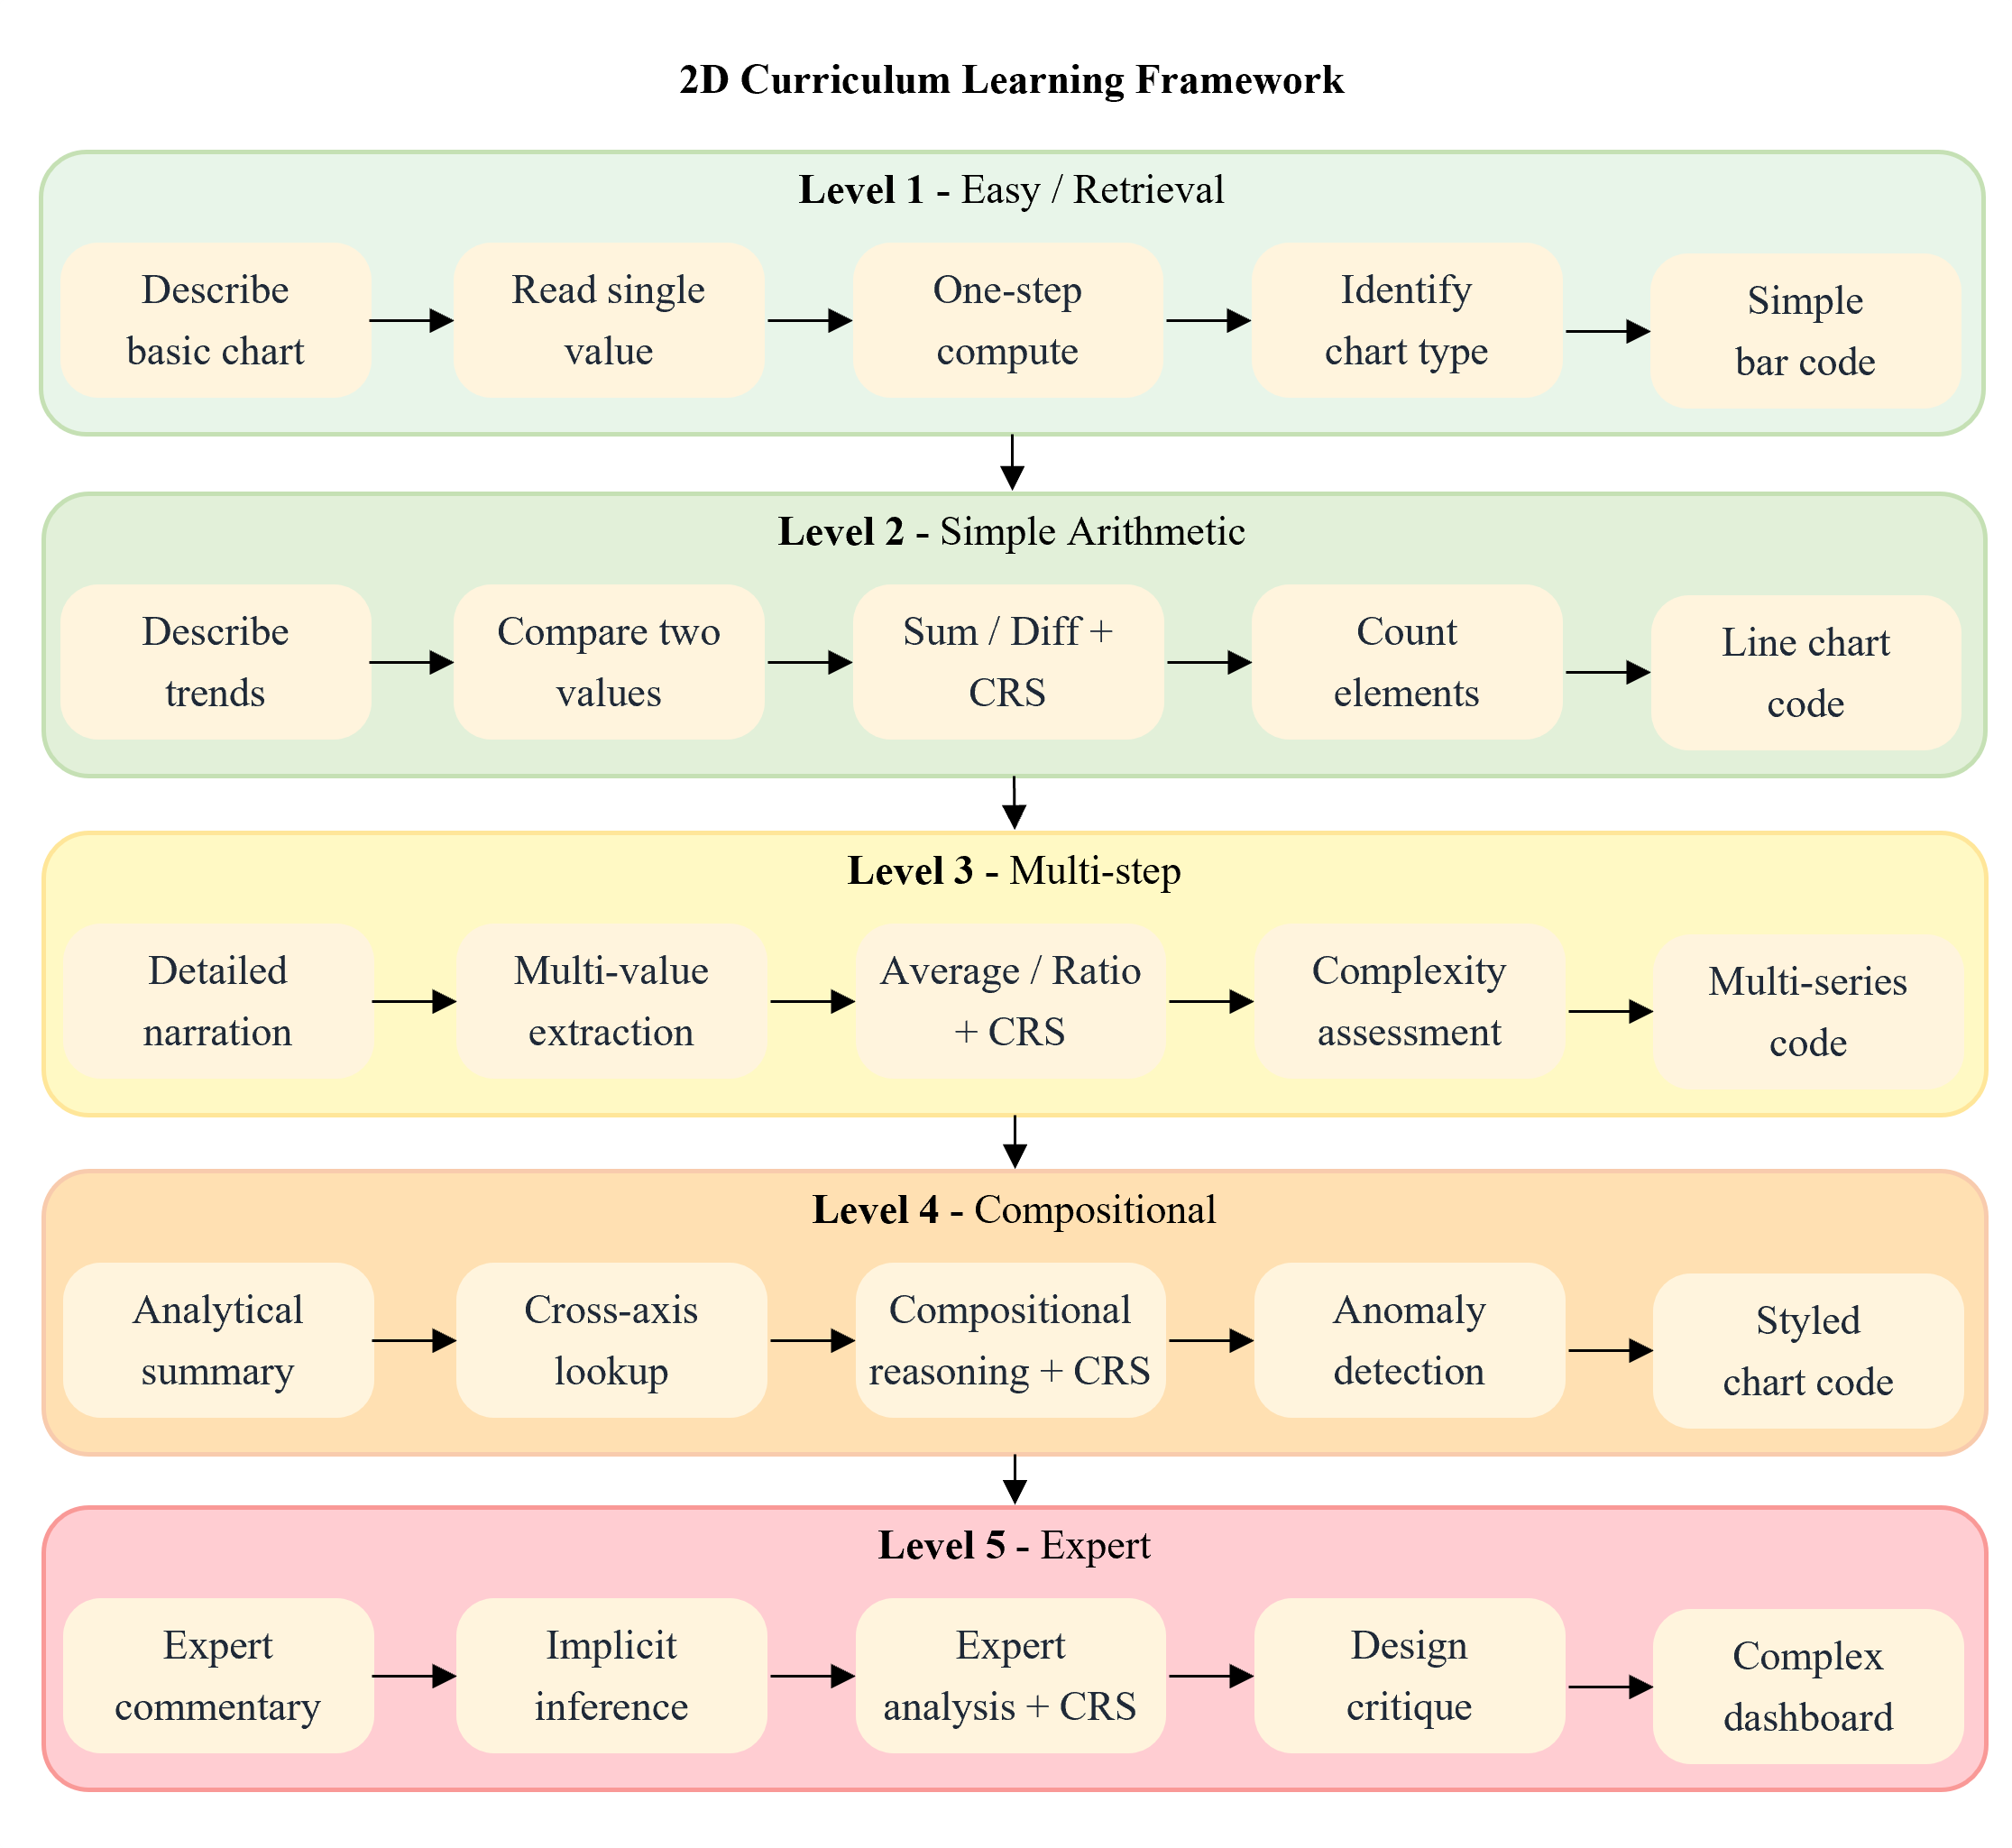
\includegraphics[width=\columnwidth]{figs/fig13_method_overview.png}
    \caption{\method{} 姒傝銆傝缁冮伒寰簩缁磋绋嬶細澶嶆潅搴﹂€掑鐨勪簲涓换鍔￠樁娈碉紝浠ュ強姣忎釜闃舵鍐呮寜闅惧害鎺掑簭鐨勬牱鏈€傞€傞厤鍣ㄦ寜椤哄簭缁ф壙锛屼粠鑰屽舰鎴愰樁娈典笓鐢ㄤ笓瀹躲€倉
    \label{fig:method_overview}
\end{figure}

鎴戜滑鐢?\textbf{\fullmethod{}锛圽method{}锛墋 瑙ｅ喅杩欎竴闂銆傝妗嗘灦鏄竴绉嶅熀浜庤绋嬪涔犵殑寰皟鏂规硶锛屾部涓や釜浜掕ˉ缁村害缁勭粐璁粌銆?
妯悜缁村害鎺у埗 \emph{浠诲姟澶嶆潅搴锛氭ā鍨嬪厛瀛︿範鍥捐〃鎻忚堪锛屽啀瀛︿範浜嬪疄闂瓟銆佹帹鐞嗛棶绛斻€佽瑙夊垎鏋愶紝鏈€鍚庡涔犱唬鐮佺敓鎴愩€?
绾靛悜缁村害鎺у埗 \emph{鏍锋湰闅惧害}锛氬湪姣忎釜闃舵鍐呴儴锛屾ā鍨嬪厛鎺ヨЕ绠€鍗曟牱鏈紝鍐嶉€愭澶勭悊鍥伴毦鏍锋湰銆?
杩欑鍒嗚В鎶婂浘琛ㄧ悊瑙ｄ粠鍗曚竴鐩爣鎷嗘垚涓€绯诲垪闅惧害閫愭澧炲姞鐨勮兘鍔涖€?

涓や釜瑕佺礌浣胯璇剧▼鏈夋晥銆?
棣栧厛锛孿textbf{浠ｇ爜鍗虫帹鐞嗙洃鐫ｏ紙\crs{}锛墋 鐢ㄥ彲鎵ц Python 杞ㄨ抗鏇夸唬涓嶉€忔槑鐨勭瓟妗堢洃鐫ｏ紝杩娇妯″瀷鍦ㄦ帹鐞嗗瘑闆嗚缁冧腑澶栧寲涓棿璁＄畻銆?
鍏舵锛孿textbf{闅惧害鎰熺煡璇剧▼鏁版嵁閫夋嫨锛圽dacds{}锛墋 浣跨敤寮鸿瑷€妯″瀷鎸夌収鎺ㄧ悊澶嶆潅搴﹀姣忎釜鏍锋湰鎺掑簭锛屼粠鑰屽湪鏃犻渶浜哄伐鏍囨敞鐨勬儏鍐典笅瀹炵幇绋冲畾鐨勭敱鏄撳埌闅捐缁冦€?

鐒惰€岋紝鍘熷澶氶樁娈佃绋嬬暀涓嬩簡涓€涓疄闄呴棶棰樸€?
濡傛灉姣忎釜闃舵閮戒細浜х敓浼樺娍涓嶅悓鐨勪笓瀹堕€傞厤鍣紝绯荤粺鍦ㄦ帹鐞嗘椂搴斿浣曢€夋嫨鍚堥€傜殑涓撳锛?
渚濊禆浜哄伐鎸囧畾閫傞厤鍣ㄦ棦涓嶆柟渚匡紝涔熸氮璐逛簡璇剧▼璁粌涓舰鎴愮殑涓撻暱銆?
鍦ㄧ幇瀹為儴缃蹭腑锛岄棶棰樺彲鑳戒粠鐩存帴鏁板€兼煡璇㈠埌缁勫悎鎺ㄧ悊鍐嶅埌缁撴瀯鍖栧浘琛ㄥ垎鏋愪笉绛夛紝鍥犳杩欎釜闂灏ゅ叾閲嶈銆?

涓鸿В鍐宠繖涓€鐐癸紝鎴戜滑寮曞叆杞婚噺绾х殑 \textbf{闃舵鎰熺煡璺敱鍣紙\sar{}锛墋銆?
缁欏畾鍥捐〃--闂瀵癸紝\sar{} 棰勬祴鏈€鍚堥€傜殑闃舵涓撳骞跺皢鏌ヨ鍒嗗彂缁欒涓撳銆?
璺敱鍣ㄤ娇鐢ㄧ敱淇濈暀楠岃瘉鏁版嵁鏋勯€犵殑 oracle 闃舵鏍囩璁粌锛屼笖鍙紩鍏ュ緢灏忕殑寤惰繜銆?
杩欐牱锛岄樁娈典笓闀夸笉鍐嶅彧鏄垎鏋愯瀵燂紝鑰屾垚涓哄彲閮ㄧ讲鐨勭郴缁熻璁°€?

鎴戜滑鐨勮瘎娴嬭寖鍥存樉钁楀浜庝細璁増銆?
% TODO-EXP-03: Replace introduction summary numbers after final experiments are fixed.
浣跨敤 Qwen2.5-VL-7B 鍜屼粎 12K 鍚堟垚鏍锋湰锛孿method{}+\sar{} 鍦?ChartQA 涓婅揪鍒?83.41\%锛屾瘮鏍囧噯 LoRA SFT 楂?7.40 涓櫨鍒嗙偣锛屾瘮鏈€浣冲崟闃舵閫傞厤鍣ㄩ珮 1.29 涓櫨鍒嗙偣銆?
杩欑鎻愬崌鍦ㄤ笁涓殢鏈虹瀛愪笅绋冲畾瀛樺湪锛屽彲杩佺Щ鍒?Qwen2.5-VL-3B 鍜?InternVL2-8B锛屽苟娉涘寲鍒?PlotQA銆丗igureQA銆丆hartBench 鍜?OpenCQA銆?
鎴戜滑杩涗竴姝ヨ〃鏄庯紝璇剧▼鍦ㄤ綆鏁版嵁鍦烘櫙涓挨鍏舵湁鐩婏紝鑳藉鍑忓皯鎺ㄧ悊閿欒鍜屾牸寮忛敊璇紝骞舵彁鍗囧浘鍍忔壈鍔ㄤ笅鐨勯瞾妫掓€с€?

鏈枃璐＄尞濡備笅锛?
\begin{itemize}
    \item 鎴戜滑鎻愬嚭涓€绉嶉潰鍚戝浘琛ㄧ悊瑙ｇ殑浜岀淮璇剧▼瀛︿範妗嗘灦锛岃仈鍚堝缓妯′换鍔″鏉傚害涓庢牱鏈毦搴︺€?
    \item 鎴戜滑寮曞叆 \crs{}锛屽苟璇佹槑鍙墽琛屼唬鐮佺洃鐫ｈ兘澶熸樉钁楁彁鍗囨帹鐞嗗瘑闆嗗瀷鍥捐〃浠诲姟銆?
    \item 鎴戜滑鎻愬嚭 \sar{}锛屼竴绉嶈交閲忔帹鐞嗘ā鍧楋紝鍙嚜鍔ㄩ€夋嫨闃舵涓撶敤閫傞厤鍣紝骞跺皢璇剧▼浜х敓鐨勪笓瀹惰兘鍔涜浆鍖栦负瀹為檯閮ㄧ讲鏈哄埗銆?
    \item 鎴戜滑鍦ㄥ涓骞叉ā鍨嬨€佹暟鎹泦銆侀殢鏈虹瀛愩€佹暟鎹妯″拰椴佹鎬ц缃笂鎻愪緵鎵╁睍璇勬祴锛岃〃鏄庤妗嗘灦鎻愬崌浜嗗噯纭巼銆佹暟鎹晥鐜囧拰閮ㄧ讲瀹炵敤鎬с€?
\end{itemize}

\section{鐩稿叧宸ヤ綔}
\paragraph{鍥捐〃鐞嗚В銆倉
鏃╂湡鍥捐〃闂瓟绯荤粺灏嗕换鍔″垎瑙ｄ负鍥捐〃瑙ｆ瀽浠ュ強闅忓悗鐨勭鍙锋垨鏂囨湰鎺ㄧ悊~\cite{kafle2018dvqa,kahou2017figureqa}銆?
杩欑被娴佹按绾胯櫧鐒跺彲瑙ｉ噴锛屼絾瀹规槗鍙楀埌璇樊浼犳挱褰卞搷銆?
杩戞湡宸ヤ綔鍒欐洿鍊惧悜浜庣鍒扮澶氭ā鎬佹灦鏋勩€?
Pix2Struct~\cite{lee2023pix2struct} 閫氳繃棰勮缁冨涔犲睆骞曠悊瑙ｏ紝MatCha~\cite{liu2023matcha} 娉ㄥ叆鏁板鎺ㄧ悊鍜屽浘琛ㄥ弽娓叉煋鑳藉姏锛孶niChart~\cite{masry2023unichart} 璁捐鍥捐〃涓撶敤棰勮缁冧换鍔★紝DePlot~\cite{liu2023deplot} 鍦ㄦ帹鐞嗗墠灏嗗浘琛ㄨ浆涓鸿〃鏍硷紝ChartLlama~\cite{han2023chartllama} 鍒欑洿鎺ュ湪鍥捐〃鏁版嵁涓婃寚浠ゅ井璋冨妯℃€?LLM銆?
杩欎簺鏂规硶琛ㄦ槑鍥捐〃鐞嗚В鍙楃泭浜庨鍩熼€傞厤锛屼絾瀹冧滑涓昏寮鸿皟妯″瀷鏋舵瀯鎴栨暟鎹妯°€?
鎴戜滑鐨勫叧娉ㄧ偣涓嶅悓锛氭垜浠爺绌堕€氳繃缁勭粐璁粌杩囩▼鏈韩鑳藉鑾峰緱澶氬皯鏀剁泭銆?

\paragraph{瑙嗚璇█妯″瀷銆倉
LLaVA~\cite{liu2024visual}銆丵wen-VL~\cite{bai2023qwen} 鍜?InternVL~\cite{chen2024internvl} 绛夐€氱敤 VLM 宸茬粡鍏峰杈冨己鐨勮瑙夊畾浣嶅拰璇█鐢熸垚鑳藉姏銆?
GPT-4V~\cite{openai2023gpt4v} 鍜?Claude 3.5~\cite{anthropic2024claude} 绛夐棴婧愮郴缁熶篃灞曠ず鍑哄緢寮虹殑闆舵牱鏈浘琛ㄧ悊瑙ｈ兘鍔涖€?
鍥犳锛屽叧閿棶棰樹笉鍐嶆槸閫氱敤 VLM 鏄惁鑳藉璇诲彇鍥捐〃锛岃€屾槸濡備綍鍦ㄤ笉杩涜澶ц妯″啀璁粌鐨勬儏鍐典笅锛岄珮鏁堝湴灏嗗畠浠€傞厤鍒板浘琛ㄤ换鍔＄殑鐗瑰畾鎺ㄧ悊缁撴瀯銆?

\paragraph{璇剧▼瀛︿範銆倉
璇剧▼瀛︿範灏嗚缁冩牱鏈粠鏄撳埌闅炬垨浠庣畝鍗曞埌澶嶆潅缁勭粐璧锋潵~\cite{bengio2009curriculum}銆?
鍏舵敹鐩婂凡缁忓湪鍥惧儚鍒嗙被銆佽嚜鐒惰瑷€鐞嗚В鍜屾洿骞挎硾鐨勮〃寰佸涔犱腑寰楀埌瑙傚療~\cite{hacohen2019power,xu2020curriculum,soviany2022curriculum}銆?
鐒惰€岋紝鍦ㄥ妯℃€佽缃腑锛屽ぇ澶氭暟璇剧▼鍙叧娉ㄥ崟涓€闅惧害姒傚康~\cite{shen2021much}銆?
鎴戜滑灏嗚绋嬪涔犳墿灞曚负鐪熸鐨勪簩缁村舰寮忥紝浣挎ā鍨嬪悓鏃舵部浠诲姟绫诲瀷鍜屼换鍔″唴闅惧害鍓嶈繘锛屽苟杩涗竴姝ヨ〃鏄庢墍寰椾笓瀹跺彲浠ラ€氳繃鎺ㄧ悊鏃惰矾鐢卞姞浠ュ埄鐢ㄣ€?

\paragraph{鎺ㄧ悊鐩戠潱涓庢ā鍧楀寲鎺ㄧ悊銆倉
閾惧紡鎬濈淮鎻愮ず鍙互璇卞鎺ㄧ悊锛屼絾涓嶆彁渚涚洿鎺ヨ缁冧俊鍙穨\cite{wei2022chain}銆?
PAL 鍜?Program-of-Thoughts 绛夌▼搴忚緟鍔╂柟娉曢€氳繃鐢熸垚浠ｇ爜澶栧寲璁＄畻~\cite{gao2023pal,chen2022program}锛岃繎鏈熷伐浣滀篃寮€濮嬫帰绱㈣瑙夊満鏅腑鐨勬樉寮忔帹鐞嗙洃鐫\cite{lu2024mathvista,shao2024visual}銆?
鎴戜滑鐨?\crs{} 灞炰簬杩欎竴鏂瑰悜锛屼絾瀹冭鐢ㄤ綔 \emph{璁粌鏃秨 鐩戠潱锛岃€屼笉鏄帹鐞嗘椂鎵ц鏈哄埗銆?
涓庢鍚屾椂锛岃澶氬疄鐢ㄧ郴缁熻秺鏉ヨ秺渚濊禆涓撻棬缁勪欢涓庤交閲忔帶鍒跺櫒銆?
鎴戜滑鐨?\sar{} 灏嗚繖涓€鎬濇兂搴旂敤浜庨€氳繃璇剧▼瀛︿範寰楀埌鐨勯樁娈典笓鐢?LoRA 涓撳锛屼娇鎺ㄧ悊鏃朵笓闂ㄥ寲涓嶄細鐗虹壊鏄撶敤鎬с€?

\section{鏂规硶}
鏈妭浠嬬粛 \fullmethod{}锛圽method{}锛夛紝鍗虫垜浠殑鍩轰簬璇剧▼瀛︿範鐨勫浘琛ㄧ悊瑙ｆ鏋讹紝浠ュ強灏嗛樁娈典笓闀胯浆鍖栦负鍙儴缃叉帹鐞嗙瓥鐣ョ殑 \sar{} 妯″潡銆?

\subsection{闂瀹氫箟}
\label{sec:problem}
缁欏畾鍥捐〃鍥惧儚 $I$ 鍜岃嚜鐒惰瑷€闂 $q$锛岀洰鏍囨槸鐢熸垚涓?$I$ 涓瑙夎瘉鎹竴鑷寸殑绛旀 $a$銆?
璇ヤ换鍔＄殑鍥伴毦鍦ㄤ簬鍥捐〃鑰﹀悎浜嗗绉嶈兘鍔涳細瑙嗚鏍囪鍜屽竷灞€璇嗗埆銆佹枃鏈笌鍥惧舰瀵归綈銆佹暟鍊艰鍙栥€佺畻鏈粍鍚堜互鍙婄瓟妗堟牸寮忓寲銆?
鍥犳锛屾垜浠笉鎶婂浘琛ㄧ悊瑙ｅ缓妯′负鍗曚竴鎶€鑳斤紝鑰屾槸寤烘ā涓轰竴缁勫彲娓愯繘瀛︿範鐨勮兘鍔涘簭鍒椼€?

\subsection{浜岀淮璇剧▼璁捐}
\label{sec:2d_curriculum}
\paragraph{妯悜缁村害锛氫换鍔″鏉傚害銆倉
鎴戜滑灏嗚缁冪粍缁囦负浜斾釜闃舵锛?
\begin{enumerate}
    \item \textbf{闃舵 1锛氬浘鍍忔弿杩般€倉 妯″瀷瀛︿範鍥捐〃绫诲瀷璇嗗埆銆佸潗鏍囪酱璇箟銆佽秼鍔挎弿杩板拰閫氱敤瑙嗚璇█瀵归綈銆?
    \item \textbf{闃舵 2锛氬熀纭€ VQA銆倉 妯″瀷鍥炵瓟鐩存帴妫€绱㈠拰绠€鍗曟瘮杈冮棶棰樸€?
    \item \textbf{闃舵 3锛氭帹鐞?VQA銆倉 妯″瀷閫氳繃 \crs{} 涓殑鏄惧紡涓棿璁＄畻澶勭悊澶氭鎺ㄧ悊銆?
    \item \textbf{闃舵 4锛氳瑙夊垎鏋愩€倉 妯″瀷鎵ц缁撴瀯鎬ф鏌ワ紝渚嬪鍏冪礌璁℃暟銆佸浘琛ㄥ垎绫诲拰甯冨眬鎰熺煡鍒嗘瀽銆?
    \item \textbf{闃舵 5锛氫唬鐮佺敓鎴愩€倉 妯″瀷鐢熸垚鍙墽琛屼唬鐮侊紝鏍规嵁搴曞眰鏁版嵁鍜岃瑙夎鏍奸噸寤哄浘琛ㄣ€?
\end{enumerate}
杩欎竴椤哄簭鍙嶆槧浜嗘暀瀛︿笂鐨勪緷璧栫粨鏋勶細鍚庣画浠诲姟寤虹珛鍦ㄦ棭鏈熸妧鑳戒箣涓娿€?

\paragraph{绾靛悜缁村害锛氭牱鏈毦搴︺€倉
鍦ㄦ瘡涓樁娈靛唴閮紝鏍锋湰鎸夌収浜旂骇闅惧害浠庢槗鍒伴毦鎺掑簭锛?
\begin{itemize}
    \item \textbf{Level 1:} 浠庡崟涓浘琛ㄥ厓绱犵洿鎺ユ绱€?
    \item \textbf{Level 2:} 瀵圭洿鎺ヨ鍙栫殑鍊艰繘琛屼竴姝ョ畻鏈€?
    \item \textbf{Level 3:} 娑夊強澶氫釜鏁板€肩殑澶氭璁＄畻銆?
    \item \textbf{Level 4:} 缁撳悎澶氱妯″紡鐨勭粍鍚堟帹鐞嗐€?
    \item \textbf{Level 5:} 闇€瑕佺粏鑷磋В閲婃垨棰嗗煙鐭ヨ瘑鐨勪笓瀹剁骇闂銆?
\end{itemize}
杩欑鐢辨槗鍒伴毦鐨勬帓搴忕ǔ瀹氫簡姣忎釜闃舵鍐呴儴鐨勪紭鍖栬繃绋嬶紝骞朵娇璇剧▼鐪熸鎴愪负浜岀淮璇剧▼锛岃€屼笉浠呬粎鏄樁娈靛紡璁粌銆?

\subsection{浠ｇ爜鍗虫帹鐞嗙洃鐫
\label{sec:crs}
瀵规帹鐞嗗瘑闆嗗瀷鍥捐〃闂鑰岃█锛屼粎浠庣瓟妗堢洃鐫ｄ腑瀛︿範寰堝洶闅撅紝鍥犱负姝ｇ‘绛旀骞朵笉鎻ず璁＄畻璺緞銆?
鎴戜滑鐢?\textbf{浠ｇ爜鍗虫帹鐞嗙洃鐫ｏ紙\crs{}锛墋 瑙ｅ喅杩欎竴闂銆?
瀵逛簬鎺ㄧ悊鏍锋湰锛屾ā鍨嬭璁粌鐢熸垚鍙墽琛?Python 杞ㄨ抗锛屾樉寮忓憟鐜版暟鍊兼娊鍙栥€佷腑闂村彉閲忓拰绠楁湳鎿嶄綔銆?
渚嬪锛岃嫢闂瑕佹眰璁＄畻涓や釜瀛ｅ害鏀跺叆涔嬪拰锛岀洃鐫ｄ俊鍙蜂細鍏堢粦瀹氫袱涓暟鍊硷紝鍐嶈绠楀畠浠殑鍜屻€?

杩欑鐩戠潱褰㈠紡鏈変笁涓紭鐐广€?
绗竴锛屽畠浣挎帹鐞嗕俊鍙锋樉寮忓寲锛岃€屼笉鏄殣钘忓湪鏈€缁堢瓟妗堜腑銆?
绗簩锛屽畠鍙互閫氳繃绋嬪簭楠岃瘉锛氬湪鏁版嵁鏋勫缓杩囩▼涓紝涓嶈兘澶嶇幇鏈熸湜绛旀鐨勪唬鐮佹牱鏈細琚繃婊ゃ€?
绗笁锛屽畠鍑忓皯浜嗚櫄鍋囨嵎寰勫涔狅紝鍥犱负妯″瀷蹇呴』閬靛惊缁撴瀯鍖栬绠楁ā鏉匡紝鑰屼笉鏄洿鎺ョ寽娴嬩竴涓湅浼煎悎鐞嗙殑鏁板瓧銆?

\paragraph{\crs{} 鐨勬帹鐞嗘柟寮忋€倉
鍦ㄥ熀鍑嗘帹鐞嗛樁娈碉紝鎴戜滑涓嶅湪澶栭儴鎵ц浠ｇ爜銆?
鐩稿弽锛岄樁娈?3 瀛﹀埌鐨勬帹鐞嗘ā寮忛€氳繃閫傞厤鍣ㄧ户鎵胯浆绉诲埌涓嬫父涓撳锛岃繖浜涗笓瀹剁敓鎴愮洿鎺ユ枃鏈瓟妗堛€?
杩欎繚鐣欎簡浠ｇ爜鐩戠潱鐨勬敹鐩婏紝鍚屾椂涓嶄細寮曞叆瀵?Python 瑙ｉ噴鍣ㄧ殑杩愯鏃朵緷璧栥€?

\subsection{闅惧害鎰熺煡璇剧▼鏁版嵁閫夋嫨}
\label{sec:dacds}
澶ц妯′汉宸ラ毦搴︽爣娉ㄥ苟涓嶇幇瀹烇紝鍥犳鎴戜滑浣跨敤 Qwen2.5-72B-Instruct 浣滀负鑷姩闅惧害璇勫垎鍣ㄣ€?
缁欏畾鍥捐〃涓婁笅鏂囥€侀棶棰樺拰绛旀锛岃瘎鍒嗗櫒鏍规嵁棰勬湡鎺ㄧ悊姝ユ暟銆佺畻鏈鏉傚害鍜岀煡璇嗛渶姹傦紝灏嗘牱鏈垎閰嶅埌 1 鍒?5 鐨勯毦搴︾瓑绾с€?
闅忓悗锛屾瘡涓樁娈电殑璁粌鏍锋湰鎸夌収璇ュ垎鏁板崌搴忔帓搴忋€?

鎴戜滑灏嗚繖涓€杩囩▼绉颁负 \textbf{闅惧害鎰熺煡璇剧▼鏁版嵁閫夋嫨锛圽dacds{}锛墋銆?
妯悜璇剧▼鍐冲畾涓嬩竴姝ュ涔?\emph{鍝} 鑳藉姏锛岃€?\dacds{} 鍐冲畾鍦ㄨ鑳藉姏鍐呴儴 \emph{濡備綍} 鎺掑垪鏍锋湰銆?

\subsection{甯﹂€傞厤鍣ㄧ户鎵跨殑娓愯繘寮忓井璋儅
\label{sec:adapter}
鎴戜滑浣跨敤 LoRA 閫傞厤鍣ㄥ疄鐜拌绋媬\cite{hu2022lora}銆?
浠?$\theta_0$ 琛ㄧず鍐荤粨鐨勯璁粌 VLM 鍙傛暟锛?\Delta\theta_s$ 琛ㄧず闃舵 $s$ 瀛﹀埌鐨?LoRA 鍙傛暟銆?
璁粌鎸夐『搴忚繘琛岋細
\begin{align}
    \Delta\theta_1 &= \text{Train}(\theta_0, \mathcal{D}_1), \\
    \Delta\theta_s &= \text{Train}(\theta_0 + \Delta\theta_{s-1}, \mathcal{D}_s), \quad s=2,\ldots,5,
\end{align}
鍏朵腑 $\mathcal{D}_s$ 鏄樁娈?$s$ 鐨勯毦搴︽帓搴忔暟鎹€?
鍏抽敭璁捐鏄?\emph{閫傞厤鍣ㄧ户鎵縸锛氭瘡涓樁娈典粠涓婁竴闃舵寮€濮嬶紝鑰屼笉鏄粠鍩虹妯″瀷閲嶆柊寮€濮嬨€?
杩欓紦鍔辩煡璇嗕粠鎻忚堪绱Н鍒版娊鍙栥€佷粠鎶藉彇绱Н鍒版帹鐞嗐€佸啀浠庢帹鐞嗙疮绉埌缁撴瀯缁煎悎銆?

鏈€缁堝緱鍒扮殑鏄竴缁勯樁娈典笓鐢ㄤ笓瀹躲€?
闃舵 2 鎿呴暱绠€娲佷簨瀹為棶绛旓紝闃舵 3 鎿呴暱鏄惧紡鎺ㄧ悊锛岄樁娈?4 鏇村彲闈犲湴澶勭悊瑙嗚瀵嗛泦闂锛岄樁娈?5 鏈€鎿呴暱缁撴瀯閲嶅缓鍜屼唬鐮佺患鍚堛€?
杩欎簺涓撳鏄竴绉嶄紭鍔匡紝浣嗕篃甯︽潵浜嗛儴缃叉寫鎴橈紝杩欐鏄笅涓€缁勪欢鐨勫姩鏈恒€?

\subsection{闃舵鎰熺煡璺敱鍣▆
\label{sec:router}
\method{} 瀛﹀埌鐨勯樁娈典笓鐢ㄩ€傞厤鍣ㄥ叿鏈変簰琛ヤ紭鍔裤€?
鎴戜滑涓嶅己杩敤鎴锋墜鍔ㄩ€夋嫨閫傞厤鍣紝鑰屾槸瀛︿範涓€涓交閲忕骇 \textbf{闃舵鎰熺煡璺敱鍣紙\sar{}锛墋锛屼负姣忎釜杈撳叆闂閫夋嫨鏈€鍚堥€傜殑涓撳銆?

缁欏畾鍥捐〃--闂瀵?$(I,q)$锛屾垜浠粠鍐荤粨楠ㄥ共涓娊鍙栨睜鍖栧妯℃€佽〃绀?$h(I,q)$锛屽苟杈撳叆涓ゅ眰鍒嗙被鍣細
\begin{align}
    p(s \mid I,q) = \text{softmax}(W_2 \sigma(W_1 h(I,q))),
\end{align}
鍏朵腑 $s \in \{2,3,4,5\}$ 琛ㄧず鍙儴缃查樁娈典笓瀹讹紝$\sigma$ 涓?GELU銆?
棰勬祴闃舵涓?
\begin{align}
    \hat{s} = \arg\max_s p(s \mid I,q).
\end{align}

\paragraph{Oracle 璺敱鏍囩銆倉
涓鸿缁?\sar{}锛屾垜浠瀯寤轰笌璇剧▼璁粌鏁版嵁涓嶉噸鍙犵殑淇濈暀璺敱闆?$\mathcal{R}$銆?
瀵?$\mathcal{R}$ 涓瘡涓牱鏈紝鎴戜滑璇勪及鎵€鏈夊彲閮ㄧ讲闃舵閫傞厤鍣紝骞跺皢 oracle 鏍囩璧嬬粰鑳戒互鏈€楂樺綊涓€鍖栫瓟妗堜技鐒剁粰鍑烘纭瓟妗堢殑闃舵銆?
鑻ュ涓樁娈甸兘姝ｇ‘锛屽垯閫夋嫨缃俊搴︽渶楂樼殑闃舵锛涜嫢鍏ㄩ儴閿欒锛屽垯鏍规嵁绮剧‘鍖归厤鍜屽綊涓€鍖栫紪杈戣窛绂诲噯鍒欙紝灏嗘爣绛捐祴缁欓敊璇渶灏忕殑闃舵銆?

\paragraph{璺敱涓轰綍鏈夋晥銆倉
璇剧▼璁粌鑷劧浜х敓涓撳锛岃€屼笉鏄崟涓€鍧囧寑妯″瀷銆?
鍩轰簬璺敱鐨勫垎鍙戝皢杩欑涓撻暱杞寲涓鸿繍琛屼紭鍔裤€?
鐩存帴鏌ュ€奸棶棰橀€氬父鐢遍樁娈?2 鍥炵瓟鏈€濂斤紝绠楁湳瀵嗛泦闂鐢遍樁娈?3 鏇撮€傚悎锛岃瑙夋嫢鎸ら棶棰樼敱闃舵 4 鏇村彲闈狅紝閲嶅缓绫婚棶棰樺垯鏇撮€傚悎闃舵 5銆?
瀹為獙琛ㄦ槑锛孿sar{} 鑳芥仮澶?oracle 璺敱鐨勫ぇ閮ㄥ垎鏀剁泭锛屽悓鏃跺彧澧炲姞寰堝皬寤惰繜銆?

\begin{figure}[!t]
    \centering
    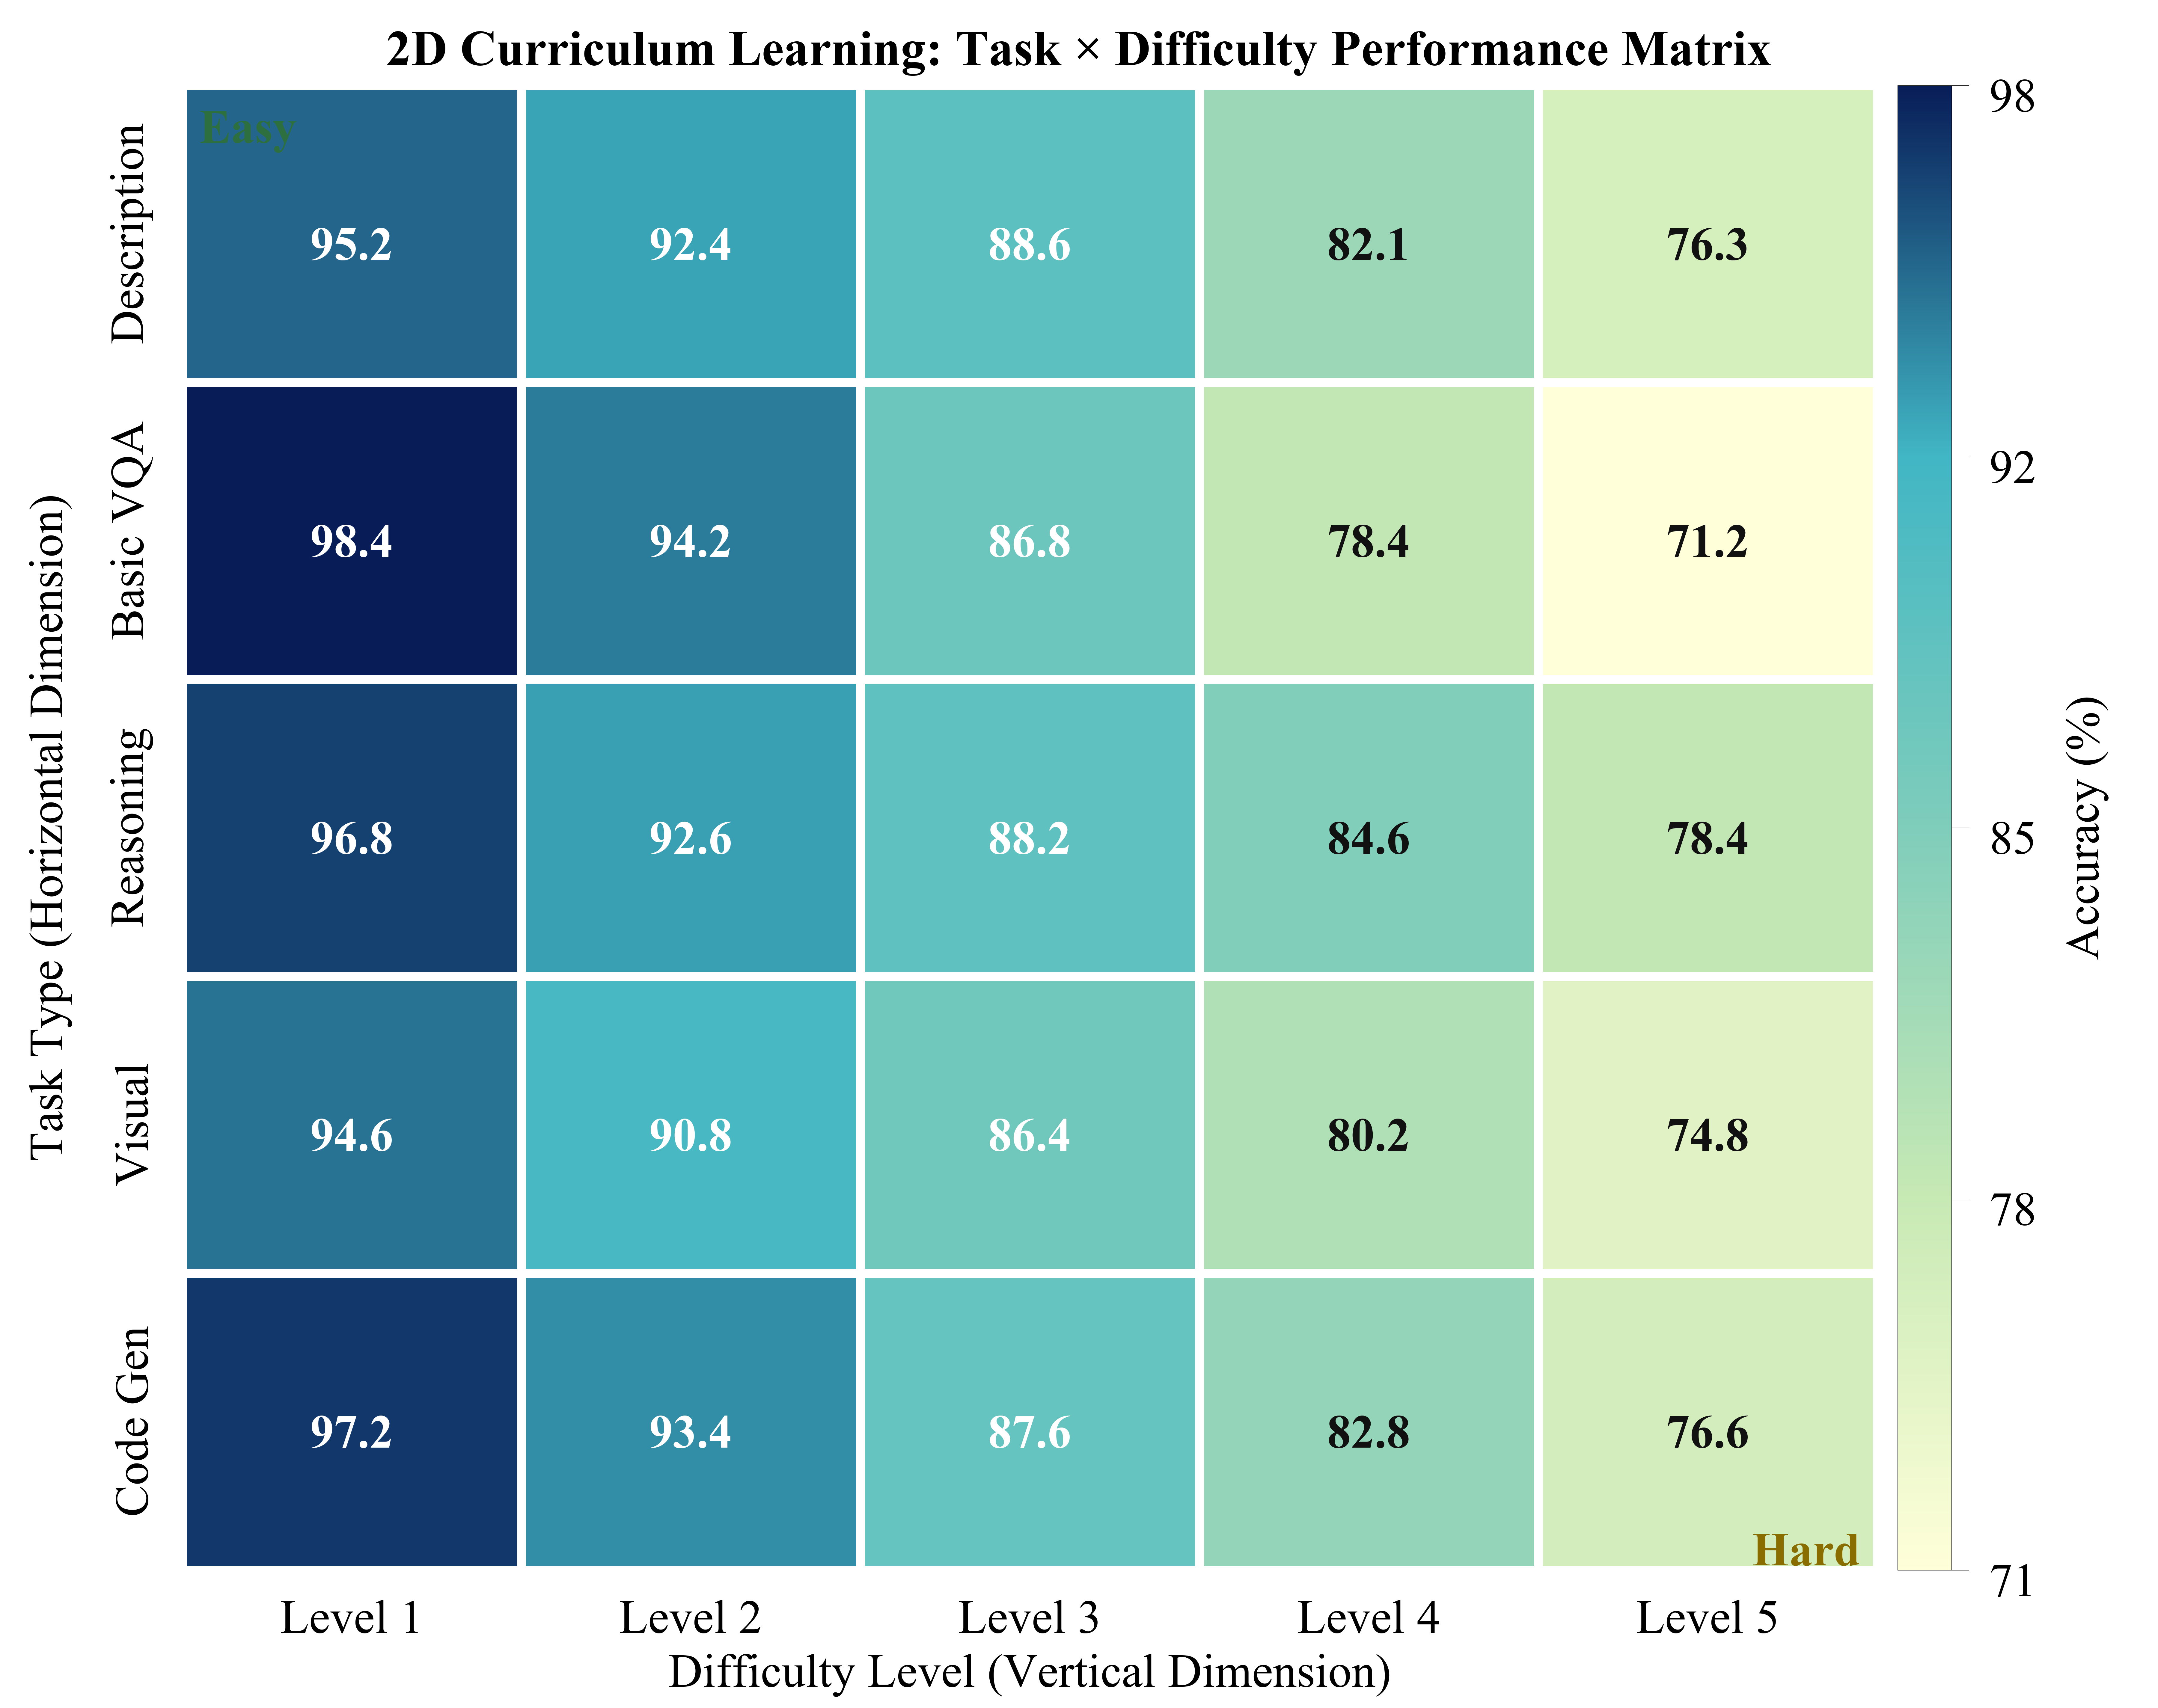
\includegraphics[width=\columnwidth]{figs/fig9_2d_curriculum_heatmap.png}
    \caption{涓嶅悓浠诲姟绫诲瀷鍜岄毦搴︾瓑绾т笂鐨勬€ц兘鐑浘銆傜畝鍗曚换鍔″噯纭巼鏈€楂橈紝骞堕殢鐫€浠诲姟鍙樹负鍥伴毦缁勫悎闂鑰岄€愭涓嬮檷锛岄獙璇佷簡浜岀淮璇剧▼鍋囪鐨勫涔犺建杩广€倉
    \label{fig:heatmap}
\end{figure}

鍥緙\ref{fig:heatmap} 鍙鍖栦簡鏈€缁堟€ц兘鍒嗗竷銆?
浠庣畝鍗?瀹规槗鍒板鏉?鍥伴毦鐨勬槑鏄惧瑙掍笅闄嶏紝鏀寔浜嗕换鍔″鏉傚害鍜屾牱鏈毦搴﹂兘鏄粍缁囧浘琛ㄥ涔犵殑鏈夋剰涔夌淮搴﹁繖涓€鍓嶆彁銆?

\section{瀹為獙}
\subsection{瀹為獙璁剧疆}
\label{sec:setup}
\paragraph{璁粌鏁版嵁銆倉
鎴戜滑浣跨敤 Python matplotlib 鐢熸垚 1,973 寮犲悎鎴愬浘琛紝瑕嗙洊 10 涓満鏅拰 5 绉嶅浘琛ㄧ被鍨嬶細鏌辩姸鍥俱€佹姌绾垮浘銆侀ゼ鍥俱€佹暎鐐瑰浘鍜岄潰绉浘銆?
瀵逛簬姣忓紶鍥撅紝Qwen2.5-72B-Instruct 鐢熸垚闃舵涓撶敤鏍囨敞锛屽寘鎷弿杩般€佷簨瀹為棶绛斿銆佹帹鐞嗛棶绛斿銆佽瑙夊垎鏋愭彁绀哄拰浠ｇ爜鐢熸垚鐩爣銆?
\crs{} 浣跨敤鐨勬帹鐞嗚建杩逛細琚墽琛屽苟鎸夋纭€ц繃婊ゃ€?
鏈€缁堣缁冮泦鍖呭惈 12,427 涓牱鏈細闃舵 1銆?銆?銆? 鍚?1,775 涓牱鏈紝闃舵 4 鍖呭惈 5,327 涓牱鏈€?
鎴戜滑棰濆淇濈暀 1,200 涓?QA 鏍锋湰锛岀敤浜庤缁冨拰楠岃瘉璺敱鍣ㄣ€?

\paragraph{鍩虹妯″瀷銆倉
涓诲疄楠屼娇鐢?Qwen2.5-VL-7B-Instruct~\cite{bai2023qwen}銆?
涓烘祴璇曟灦鏋勯瞾妫掓€э紝鎴戜滑涔熷皢鏂规硶搴旂敤浜?Qwen2.5-VL-3B-Instruct 鍜?InternVL2-8B~\cite{chen2024internvl}銆?

\paragraph{璁粌閰嶇疆銆倉
鎵€鏈夋ā鍨嬪潎浣跨敤 LoRA~\cite{hu2022lora}锛宺ank 涓?8锛?\alpha=16$锛宒ropout 涓?0.1锛屾湁鏁?batch size 涓?16銆?
闃舵 1 鍒伴樁娈?5 鐨勫涔犵巼鍒嗗埆涓?$1\times10^{-4}$銆?5\times10^{-5}$銆?3\times10^{-5}$銆?3\times10^{-5}$ 鍜?$2\times10^{-5}$銆?
姣忎釜闃舵璁粌 10 涓?epoch銆?
\sar{} 鍒嗙被鍣ㄦ槸涓€涓袱灞?MLP锛屽湪鍐荤粨澶氭ā鎬佸祵鍏ヤ笂璁粌 5 涓?epoch锛屽涔犵巼涓?$1\times10^{-4}$銆?
闄ら潪鍙︽湁璇存槑锛屾墍鏈夌粨鏋滃潎涓轰笁涓殢鏈虹瀛愮殑骞冲潎鍊笺€?

\paragraph{璇勬祴鍩哄噯銆倉
鎴戜滑浠?ChartQA~\cite{masry2022chartqa} 涓轰富瑕佸熀鍑嗐€?
杩涗竴姝ユ祴璇曞埌 PlotQA~\cite{methani2020plotqa} 鍜?FigureQA~\cite{kahou2017figureqa} 鐨勯浂鏍锋湰杩佺Щ锛屽苟鍦?ChartBench 鍜?OpenCQA 涓や釜棰濆鍩哄噯涓婅瘎浼版洿骞挎硾鐨勬硾鍖栬兘鍔涖€?
瀵逛簬椴佹鎬у垎鏋愶紝鎴戜滑鏋勯€犲甫 JPEG 鍘嬬缉銆侀珮鏂ā绯娿€佷笅閲囨牱銆侀鑹叉壈鍔ㄥ拰灞€閮ㄩ伄鎸＄殑 ChartQA 閫€鍖栫増鏈€?

\paragraph{鍩虹嚎銆倉
鎴戜滑姣旇緝鍐荤粨闆舵牱鏈熀纭€妯″瀷銆佸湪鐩稿悓 12K 鏍锋湰涓婄殑鏍囧噯 LoRA SFT銆佷袱涓竴缁磋绋嬶紙浠呬换鍔″拰浠呴毦搴︼級銆乗method{} 涓殑鏈€浣冲崟闃舵閫傞厤鍣ㄣ€乷racle 璺敱浠ュ強鏈枃鎻愬嚭鐨勯娴嬭矾鐢卞櫒銆?

\subsection{涓荤粨鏋渳
\label{sec:main_results}
% TODO-EXP-04: Replace Table~\ref{tab:sota} with real main-results numbers.
\begin{table}[!t]
\centering
\small
\begin{tabular}{lccc}
\toprule
\textbf{鏂规硶} & \textbf{鍙傛暟閲弣 & \textbf{璁粌鏁版嵁} & \textbf{ChartQA} \\
\midrule
\multicolumn{4}{l}{\textit{闂簮妯″瀷}} \\
Claude 3.5 Sonnet & --- & --- & 90.8 \\
GPT-4V & --- & --- & 85.7 \\
\midrule
\multicolumn{4}{l}{\textit{寮€婧?VLM锛坺ero-shot锛墋} \\
Qwen2.5-VL-72B & 72B & --- & 89.5 \\
InternVL2-Pro & 40B & --- & 83.8 \\
LLaVA-1.6-34B & 34B & --- & 68.3 \\
\midrule
\multicolumn{4}{l}{\textit{鍥捐〃涓撶敤妯″瀷}} \\
ChartLlama & 13B & 160K & 69.4 \\
MatCha & 282M & $\sim$2M & 64.2 \\
UniChart & 140M & 611K & 60.8 \\
Pix2Struct & 282M & 80M & 56.0 \\
DePlot & 282M & $\sim$2M & 54.3 \\
\midrule
Qwen2.5-VL-7B (zero-shot) & 7B & --- & 80.28 \\
Standard LoRA SFT & 7B & 12K & 76.01 \\
\textbf{Ours (\method{}+\sar{})} & \textbf{7B} & \textbf{12K} & \textbf{83.41} \\
\bottomrule
\end{tabular}
\caption{ChartQA 涓婄殑姣旇緝銆傚畬鏁寸郴缁熶粎浣跨敤 12K 鍚堟垚鍥捐〃鏍锋湰锛屽氨姣旀爣鍑?LoRA SFT 楂?7.40 涓櫨鍒嗙偣銆倉
\label{tab:sota}
\end{table}

% TODO-EXP-05: Replace the main-results narrative numbers in this paragraph.
琛▇\ref{tab:sota} 琛ㄦ槑锛屾墍鎻愬嚭鏂规硶鍏锋湁寰堥珮鐨勬暟鎹晥鐜囥€?
浠呬娇鐢?12K 鍚堟垚鏍锋湰鏃讹紝\method{}+\sar{} 灏辫秴杩囦簡浣跨敤鏇村ぇ瑙勬ā鍥捐〃璇枡璁粌鐨勫浘琛ㄤ笓鐢ㄧ郴缁燂紝骞舵瘮鏍囧噯 LoRA SFT 楂?7.40 涓櫨鍒嗙偣銆?
鐩告瘮鍐荤粨鐨勯浂鏍锋湰 Qwen2.5-VL-7B 鍩虹嚎锛岃绋嬪涔犲姞璺敱甯︽潵 3.13 涓櫨鍒嗙偣鎻愬崌锛岃鏄庡嵆浣垮熀纭€妯″瀷宸茬粡寰堝己锛岀粨鏋勫寲閫傞厤浠嶇劧鏈変环鍊笺€?

% TODO-EXP-06: Replace Table~\ref{tab:transfer} with real cross-dataset results.
\begin{table}[!t]
\centering
\small
\begin{tabular}{lcccc}
\toprule
\textbf{鏁版嵁闆唥 & \textbf{Std. SFT} & \textbf{鏈€浣抽樁娈祡 & \textbf{\method{}+\sar{}} & \textbf{$\Delta$} \\
\midrule
ChartQA & 76.01 & 82.12 & 83.41 & +7.40 \\
PlotQA & 52.40 & 56.71 & 58.20 & +5.80 \\
FigureQA & 90.00 & 92.11 & 93.10 & +3.10 \\
ChartBench & 68.10 & 72.82 & 74.60 & +6.50 \\
OpenCQA & 62.70 & 67.38 & 69.30 & +6.60 \\
\bottomrule
\end{tabular}
\caption{璺ㄦ暟鎹泦璇勬祴銆傛墍鎻愬嚭绯荤粺鍦ㄦ墍鏈夊熀鍑嗕笂鍧囩ǔ瀹氫紭浜庢爣鍑?SFT锛屽悓鏃朵篃瓒呰繃浜哄伐閫夋嫨鐨勬渶浣冲崟闃舵閫傞厤鍣ㄣ€倉
\label{tab:transfer}
\end{table}

% TODO-EXP-07: Replace the cross-dataset interpretation after real results are available.
琛▇\ref{tab:transfer} 灏嗚瘎娴嬫墿灞曞埌 ChartQA 涔嬪銆?
澧炵泭鍦ㄧ瀛﹀浘琛紙PlotQA锛夈€佸悎鎴愪簩鍊煎浘琛ㄩ棶绛旓紙FigureQA锛変互鍙婁袱涓洿骞挎硾鐨勫浘琛ㄦ帹鐞嗗熀鍑嗭紙ChartBench 鍜?OpenCQA锛変笂鎸佺画瀛樺湪銆?
杩欑涓€鑷存€ц〃鏄庯紝璇剧▼骞堕潪浠呬粎浼樺寲鏌愪釜鏁版嵁闆嗙殑绛旀鏍煎紡锛岃€屾槸鍦ㄥ涔犲彲杩佺Щ鑳藉姏銆?

\subsection{娑堣瀺瀹為獙}
\label{sec:ablation}
% TODO-EXP-08: Replace Table~\ref{tab:ablation} with real ablation results.
\begin{table}[!t]
\centering
\small
\begin{tabular}{lcccccc}
\toprule
\textbf{閰嶇疆} & \textbf{闃舵} & \textbf{闅惧害} & \textbf{CRS} & \textbf{缁ф壙} & \textbf{璺敱} & \textbf{Acc.} \\
\midrule
Full \method{}+\sar{} & \checkmark & \checkmark & \checkmark & \checkmark & \checkmark & 83.41 \\
\midrule
w/o Router & \checkmark & \checkmark & \checkmark & \checkmark & --- & 82.12 \\
w/o Staging & --- & \checkmark & \checkmark & --- & --- & 79.18 \\
w/o Difficulty & \checkmark & --- & \checkmark & \checkmark & --- & 81.27 \\
w/o CRS & \checkmark & \checkmark & --- & \checkmark & --- & 80.11 \\
w/o Inheritance & \checkmark & \checkmark & \checkmark & --- & --- & 77.86 \\
\midrule
Standard LoRA SFT & --- & --- & --- & --- & --- & 76.01 \\
\bottomrule
\end{tabular}
\caption{ChartQA 涓婄殑娑堣瀺瀹為獙銆傛瘡涓粍浠堕兘鏈夋鍚戣础鐚紝鍏朵腑閫傞厤鍣ㄧ户鎵垮拰浠诲姟闃舵鍖栧甫鏉ユ渶澶ф敹鐩婏紱\sar{} 鐩告瘮鏈€浣冲崟闃舵閫傞厤鍣ㄨ繘涓€姝ユ彁鍗?1.29 涓櫨鍒嗙偣銆倉
\label{tab:ablation}
\end{table}

% TODO-EXP-09: Replace ablation gains and component-importance statements with real values.
琛▇\ref{tab:ablation} 涓殑娑堣瀺缁撴灉寮哄寲浜嗕笁涓粨璁恒€?
绗竴锛岄€傞厤鍣ㄧ户鎵夸粛鐒舵槸鏈€閲嶈鐨勮缁冪粍浠讹細绉婚櫎瀹冧細鎹熷け 5.55 涓櫨鍒嗙偣銆?
绗簩锛屼换鍔￠樁娈靛寲涓庨樁娈靛唴闅惧害鎺掑簭閮藉緢閲嶈锛岃鏄庤绋嬬‘瀹炴槸浜岀淮鐨勩€?
绗笁锛孿sar{} 鍦ㄨ缁冨畬鎴愬悗棰濆甯︽潵 1.29 涓櫨鍒嗙偣鏀剁泭锛岃〃鏄庡彧鏈夊皢闃舵涓撻暱杞寲涓烘帹鐞嗙瓥鐣ユ椂锛屽畠鎵嶇湡姝ｆ湁鐢ㄣ€?

\paragraph{涓庝竴缁磋绋嬬殑姣旇緝銆倉
\emph{w/o Difficulty} 琛屽搴斾粎浠诲姟璇剧▼锛岃€?\emph{w/o Staging} 瀵瑰簲浠呴毦搴﹁绋嬨€?
% TODO-EXP-10: Replace the 1D-vs-2D comparison chain with real final values.
瀹屾暣閫掕繘鍏崇郴涓猴細
\begin{align*}
\text{2D-CL+SAR } (83.41) &> \text{ 2D-CL } (82.12) \\
&> \text{ 1D-Task } (81.27) \\
&> \text{ 1D-Difficulty } (79.18) \\
&> \text{ SFT } (76.01).
\end{align*}
浠诲姟鍒嗚В姣斿崟绾毦搴︽帓搴忓甫鏉ユ洿澶ф敹鐩婏紝浣嗗畬鏁翠簩缁磋绋嬩骇鐢熸渶浣冲崟闃舵涓撳锛岃€岃矾鐢辫繘涓€姝ュ皢鍏惰浆鍖栦负鏈€浣虫暣浣撶郴缁熴€?

\subsection{澶氶殢鏈虹瀛愪笌璺ㄦā鍨嬬粨鏋渳
% TODO-EXP-11: Replace Table~\ref{tab:seeds} with real multi-seed statistics.
\begin{table}[!t]
\centering
\small
\begin{tabular}{lc}
\toprule
\textbf{鏂规硶} & \textbf{ChartQA锛堝潎鍊?$\pm$ 鏍囧噯宸級} \\
\midrule
Standard LoRA SFT & 76.01 $\pm$ 0.31 \\
1D-Difficulty & 79.18 $\pm$ 0.28 \\
1D-Task & 81.27 $\pm$ 0.26 \\
\method{} (best single stage) & 82.12 $\pm$ 0.24 \\
\method{}+\sar{} & 83.41 $\pm$ 0.18 \\
\bottomrule
\end{tabular}
\caption{ChartQA 涓婄殑涓夐殢鏈虹瀛愯瘎娴嬨€俓method{}+\sar{} 鐩告瘮鏍囧噯 SFT 鐨勬彁鍗囩ǔ瀹氬瓨鍦紝涓旈殢鐫€璇剧▼缁撴瀯澧炲己锛屾柟宸€愭鍑忓皬銆倉
\label{tab:seeds}
\end{table}

\begin{figure*}[!t]
    \centering
    \subfloat[娑堣瀺瀹為獙]{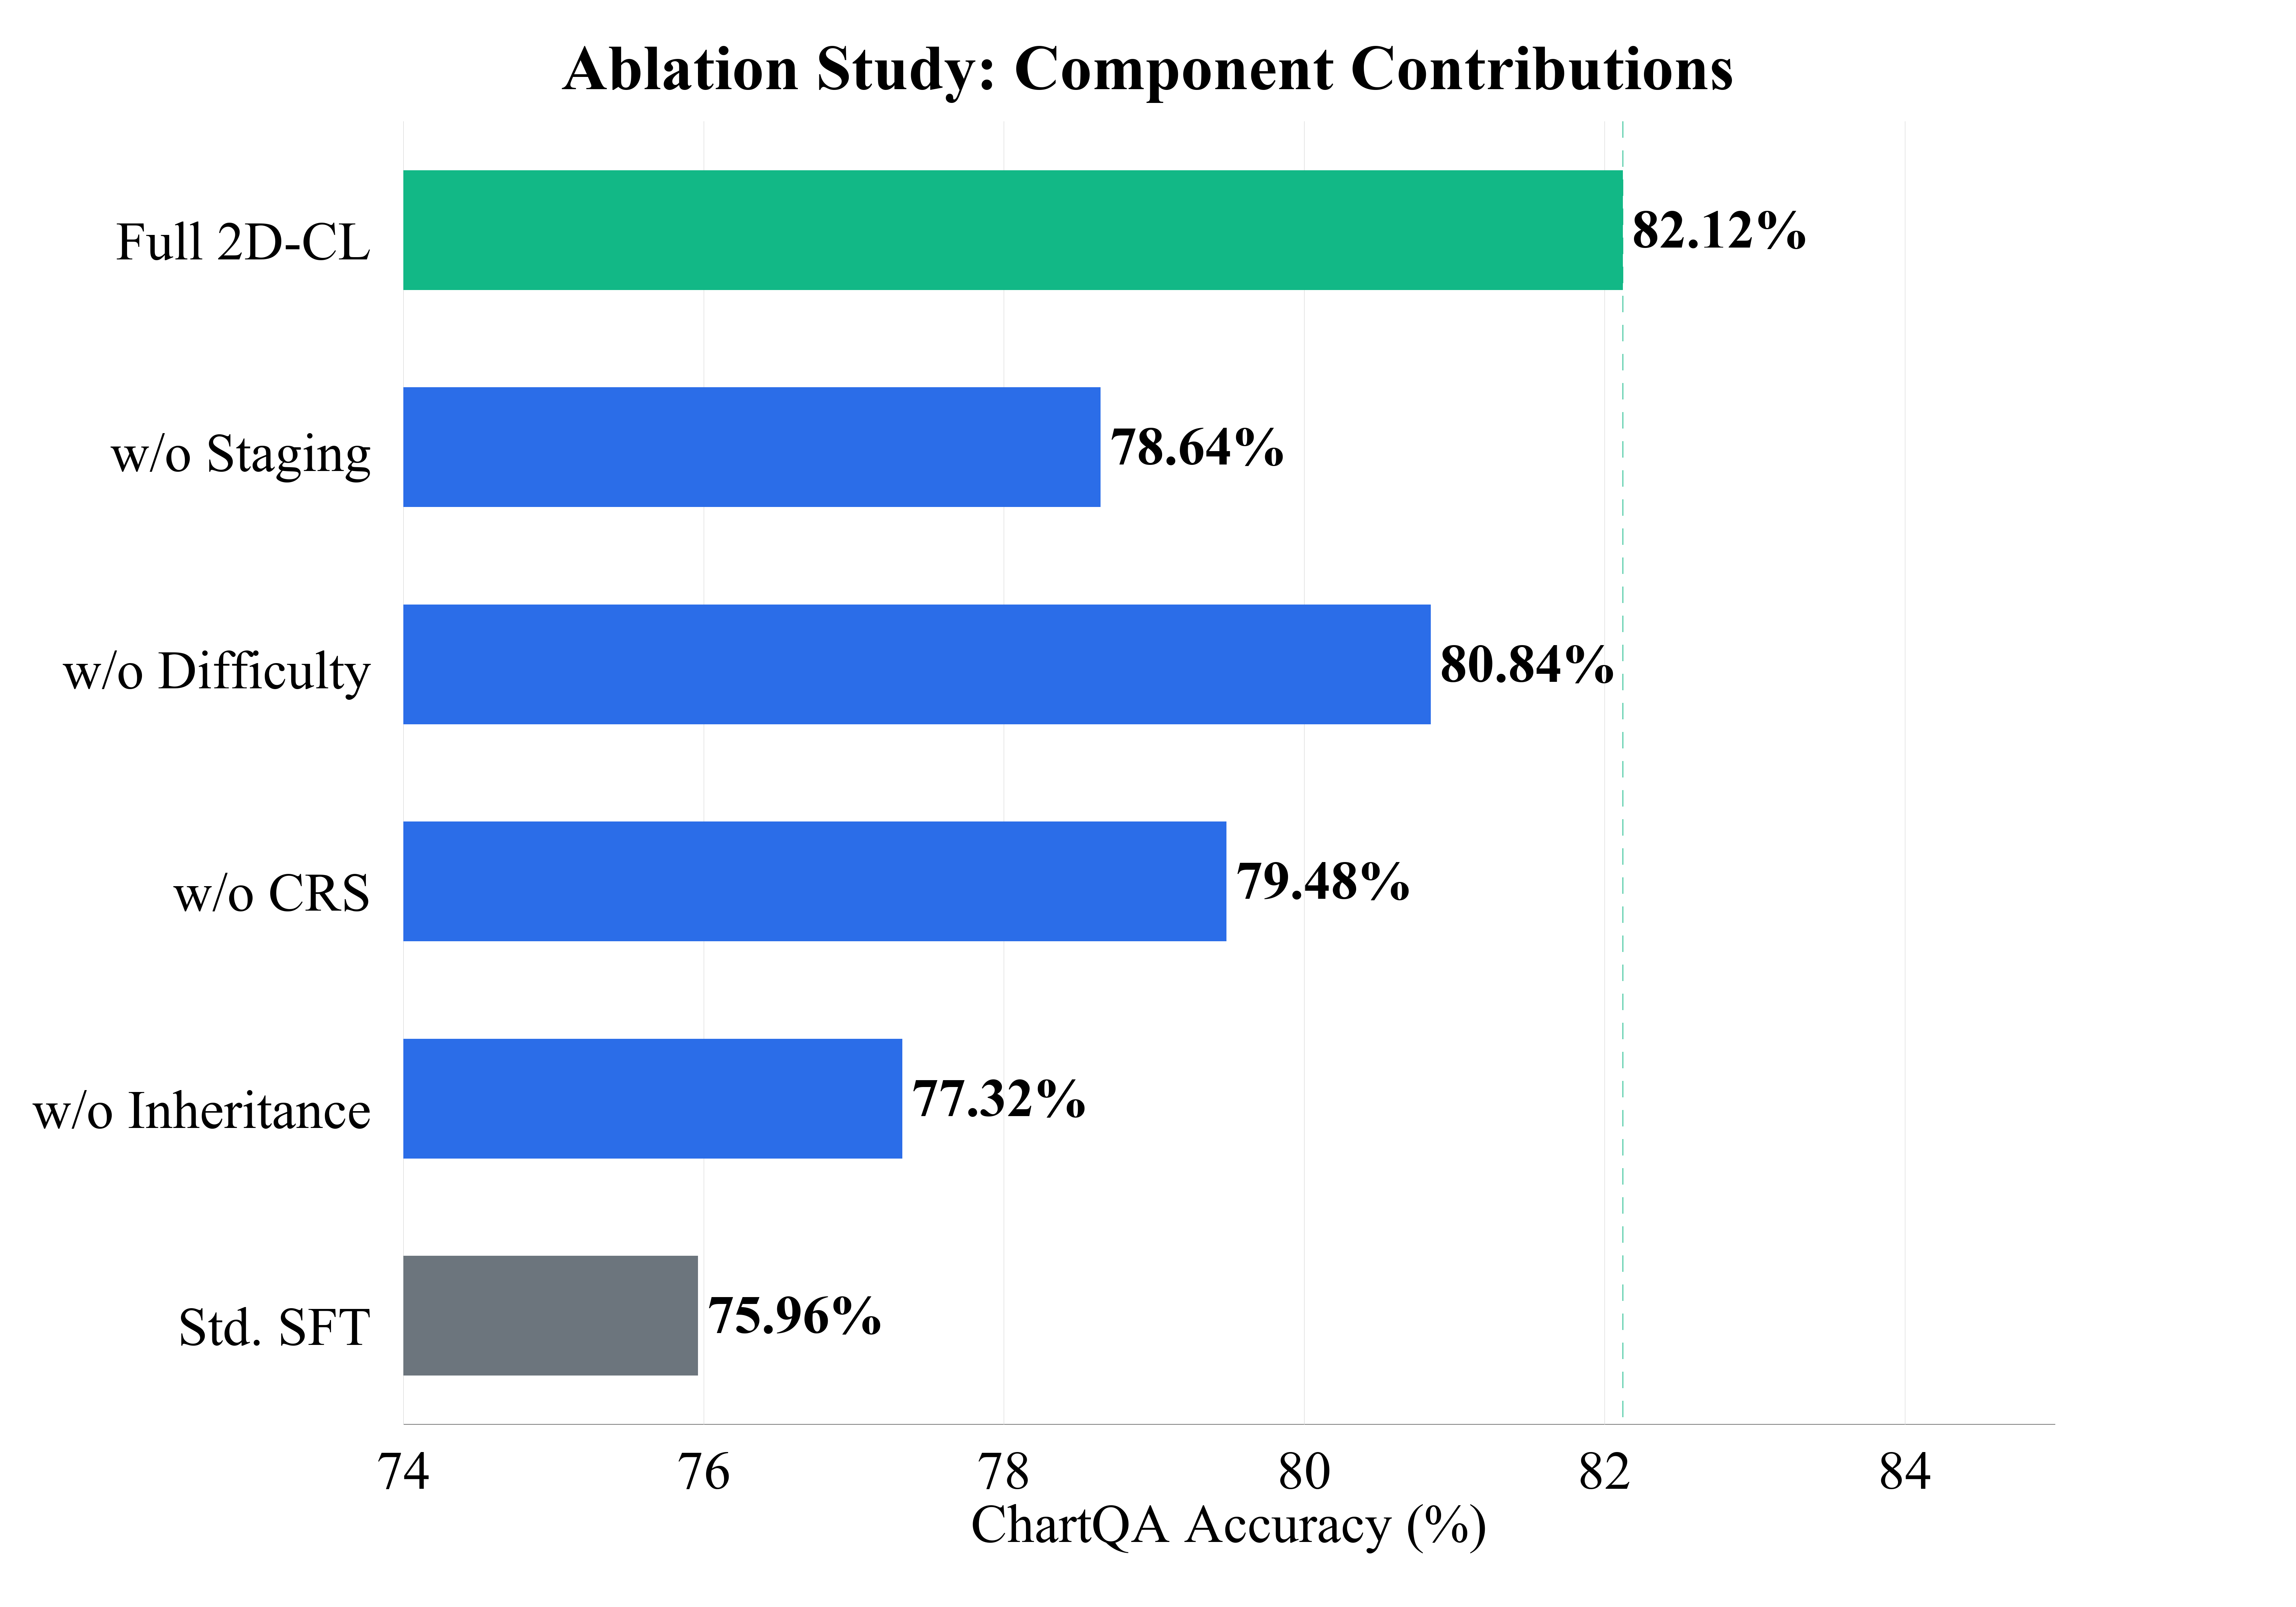
\includegraphics[width=0.32\textwidth]{figs/fig3_ablation_study.png}\label{fig:exp_ablation}}
    \hfil
    \subfloat[璺ㄦā鍨嬫硾鍖朷{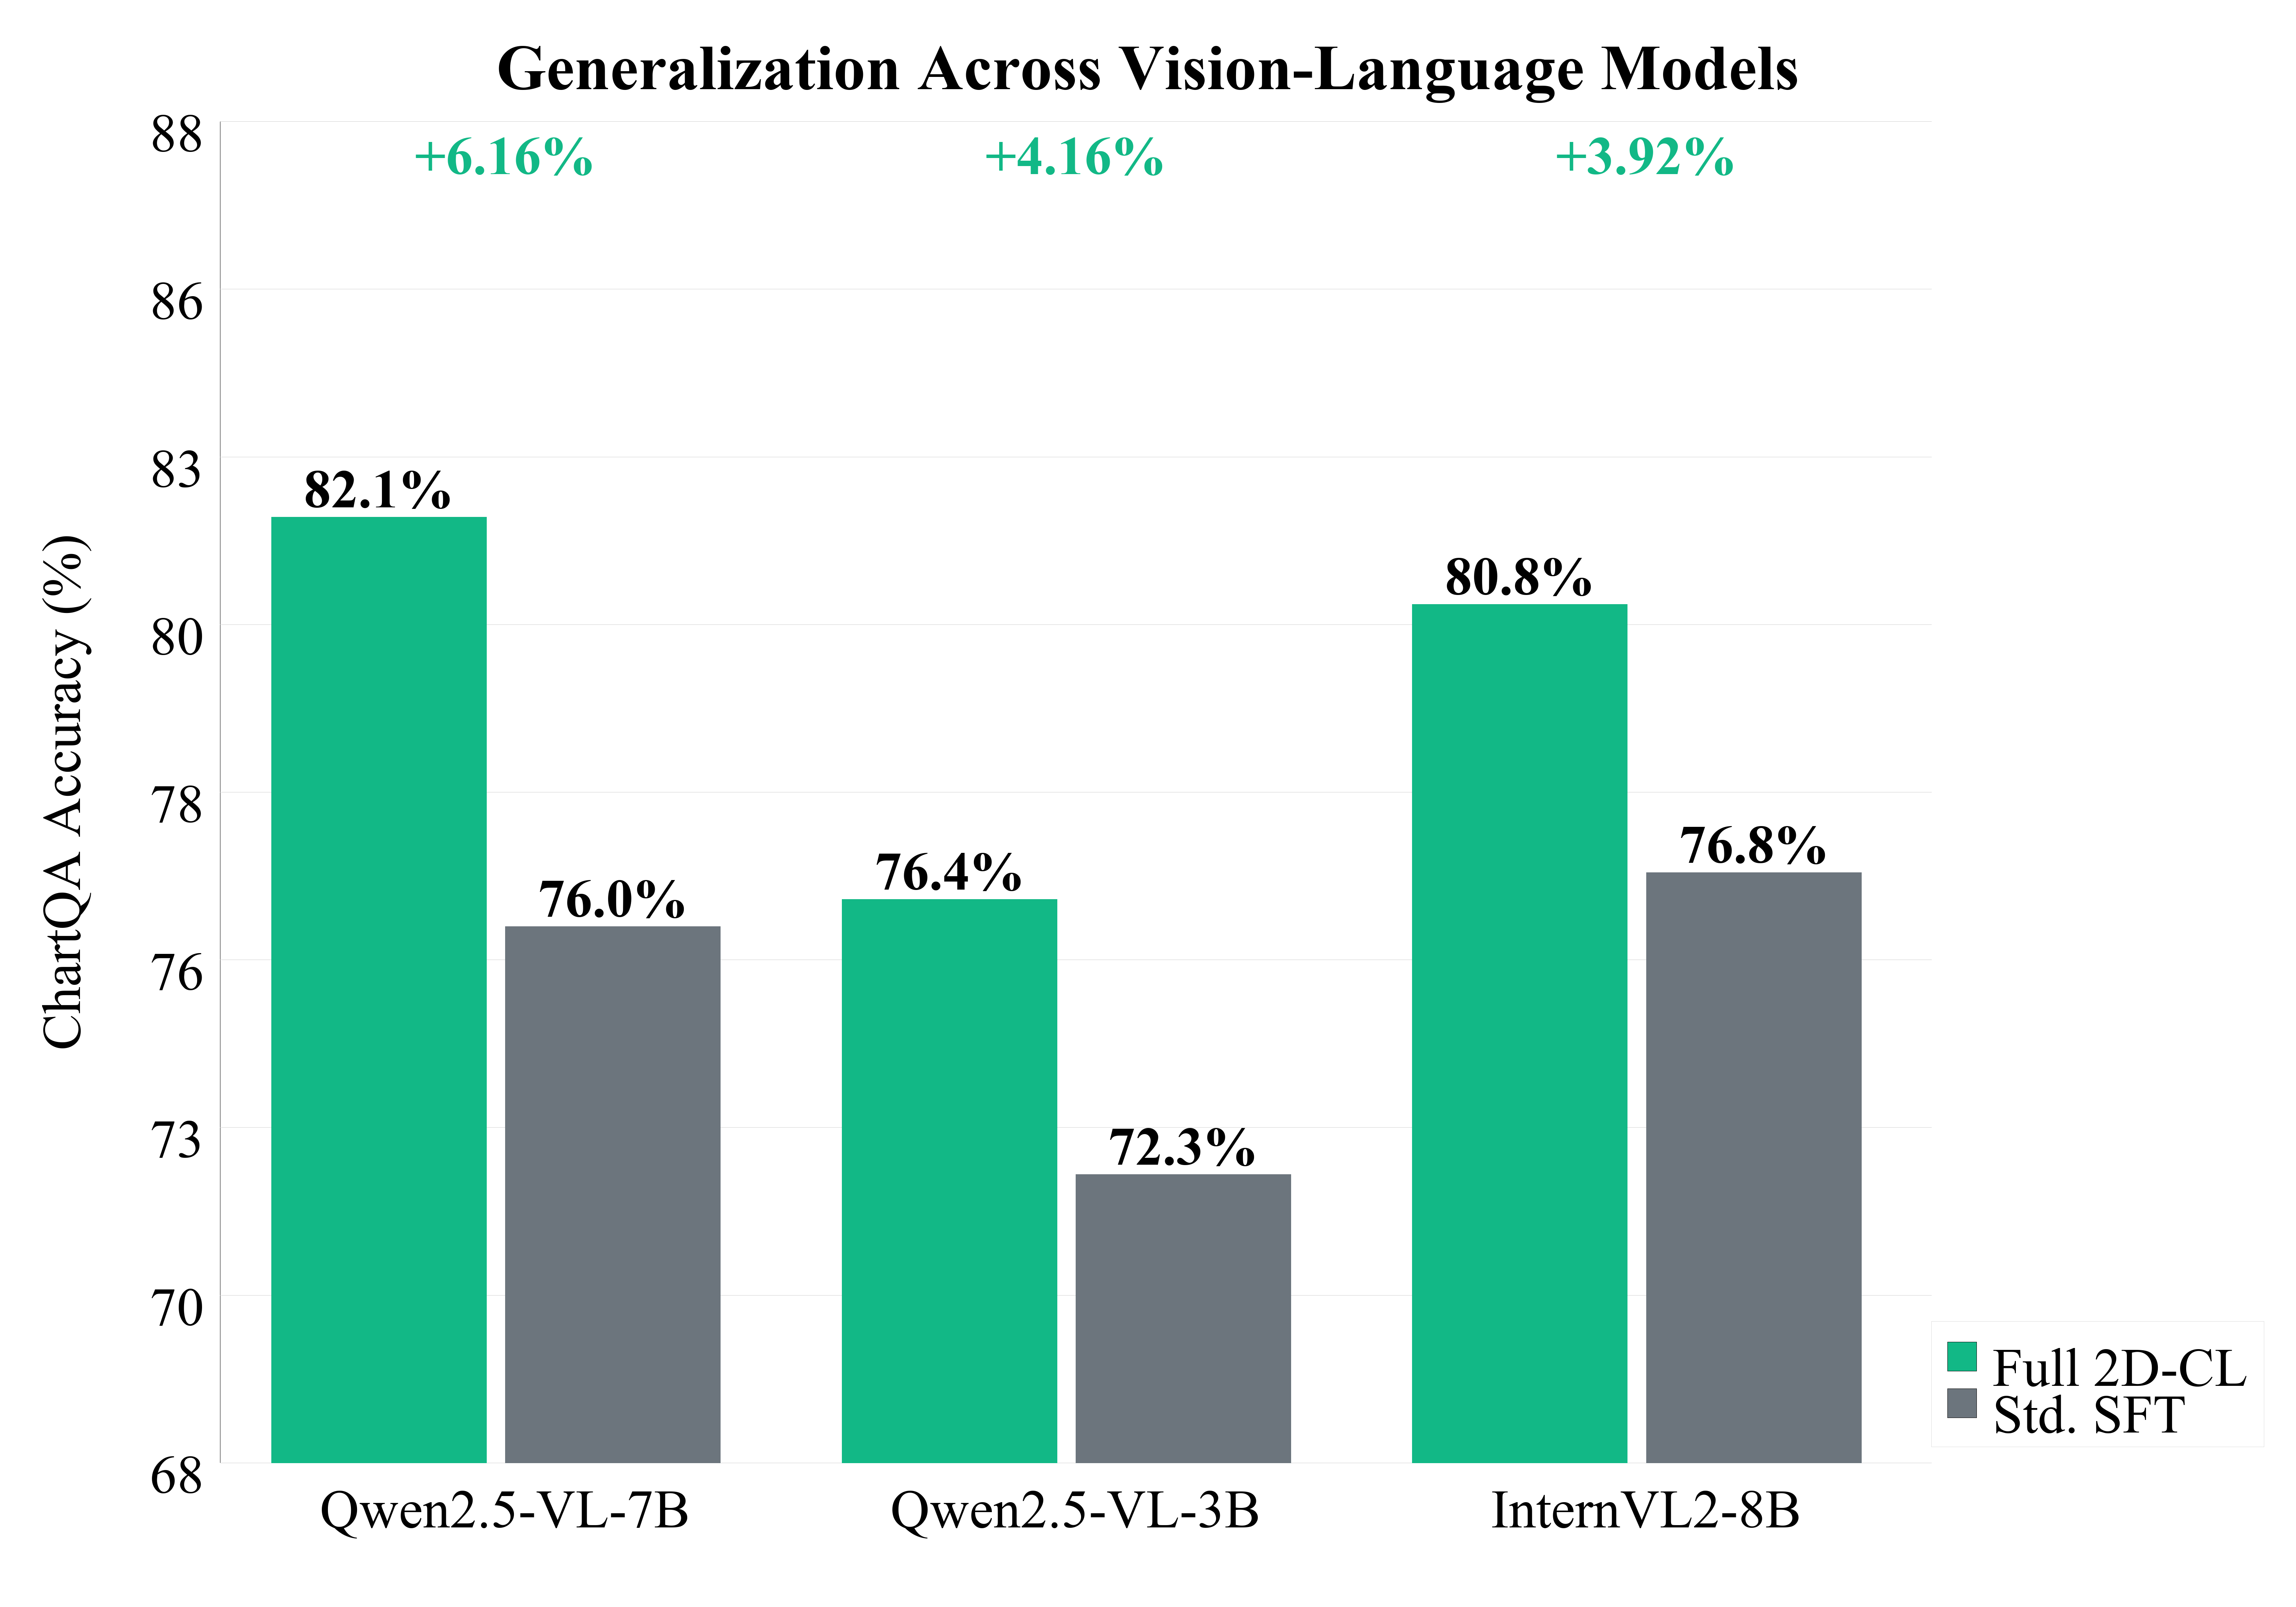
\includegraphics[width=0.32\textwidth]{figs/fig5_multi_model_comparison.png}\label{fig:exp_models}}
    \hfil
    \subfloat[璺ㄦ暟鎹泦杩佺Щ]{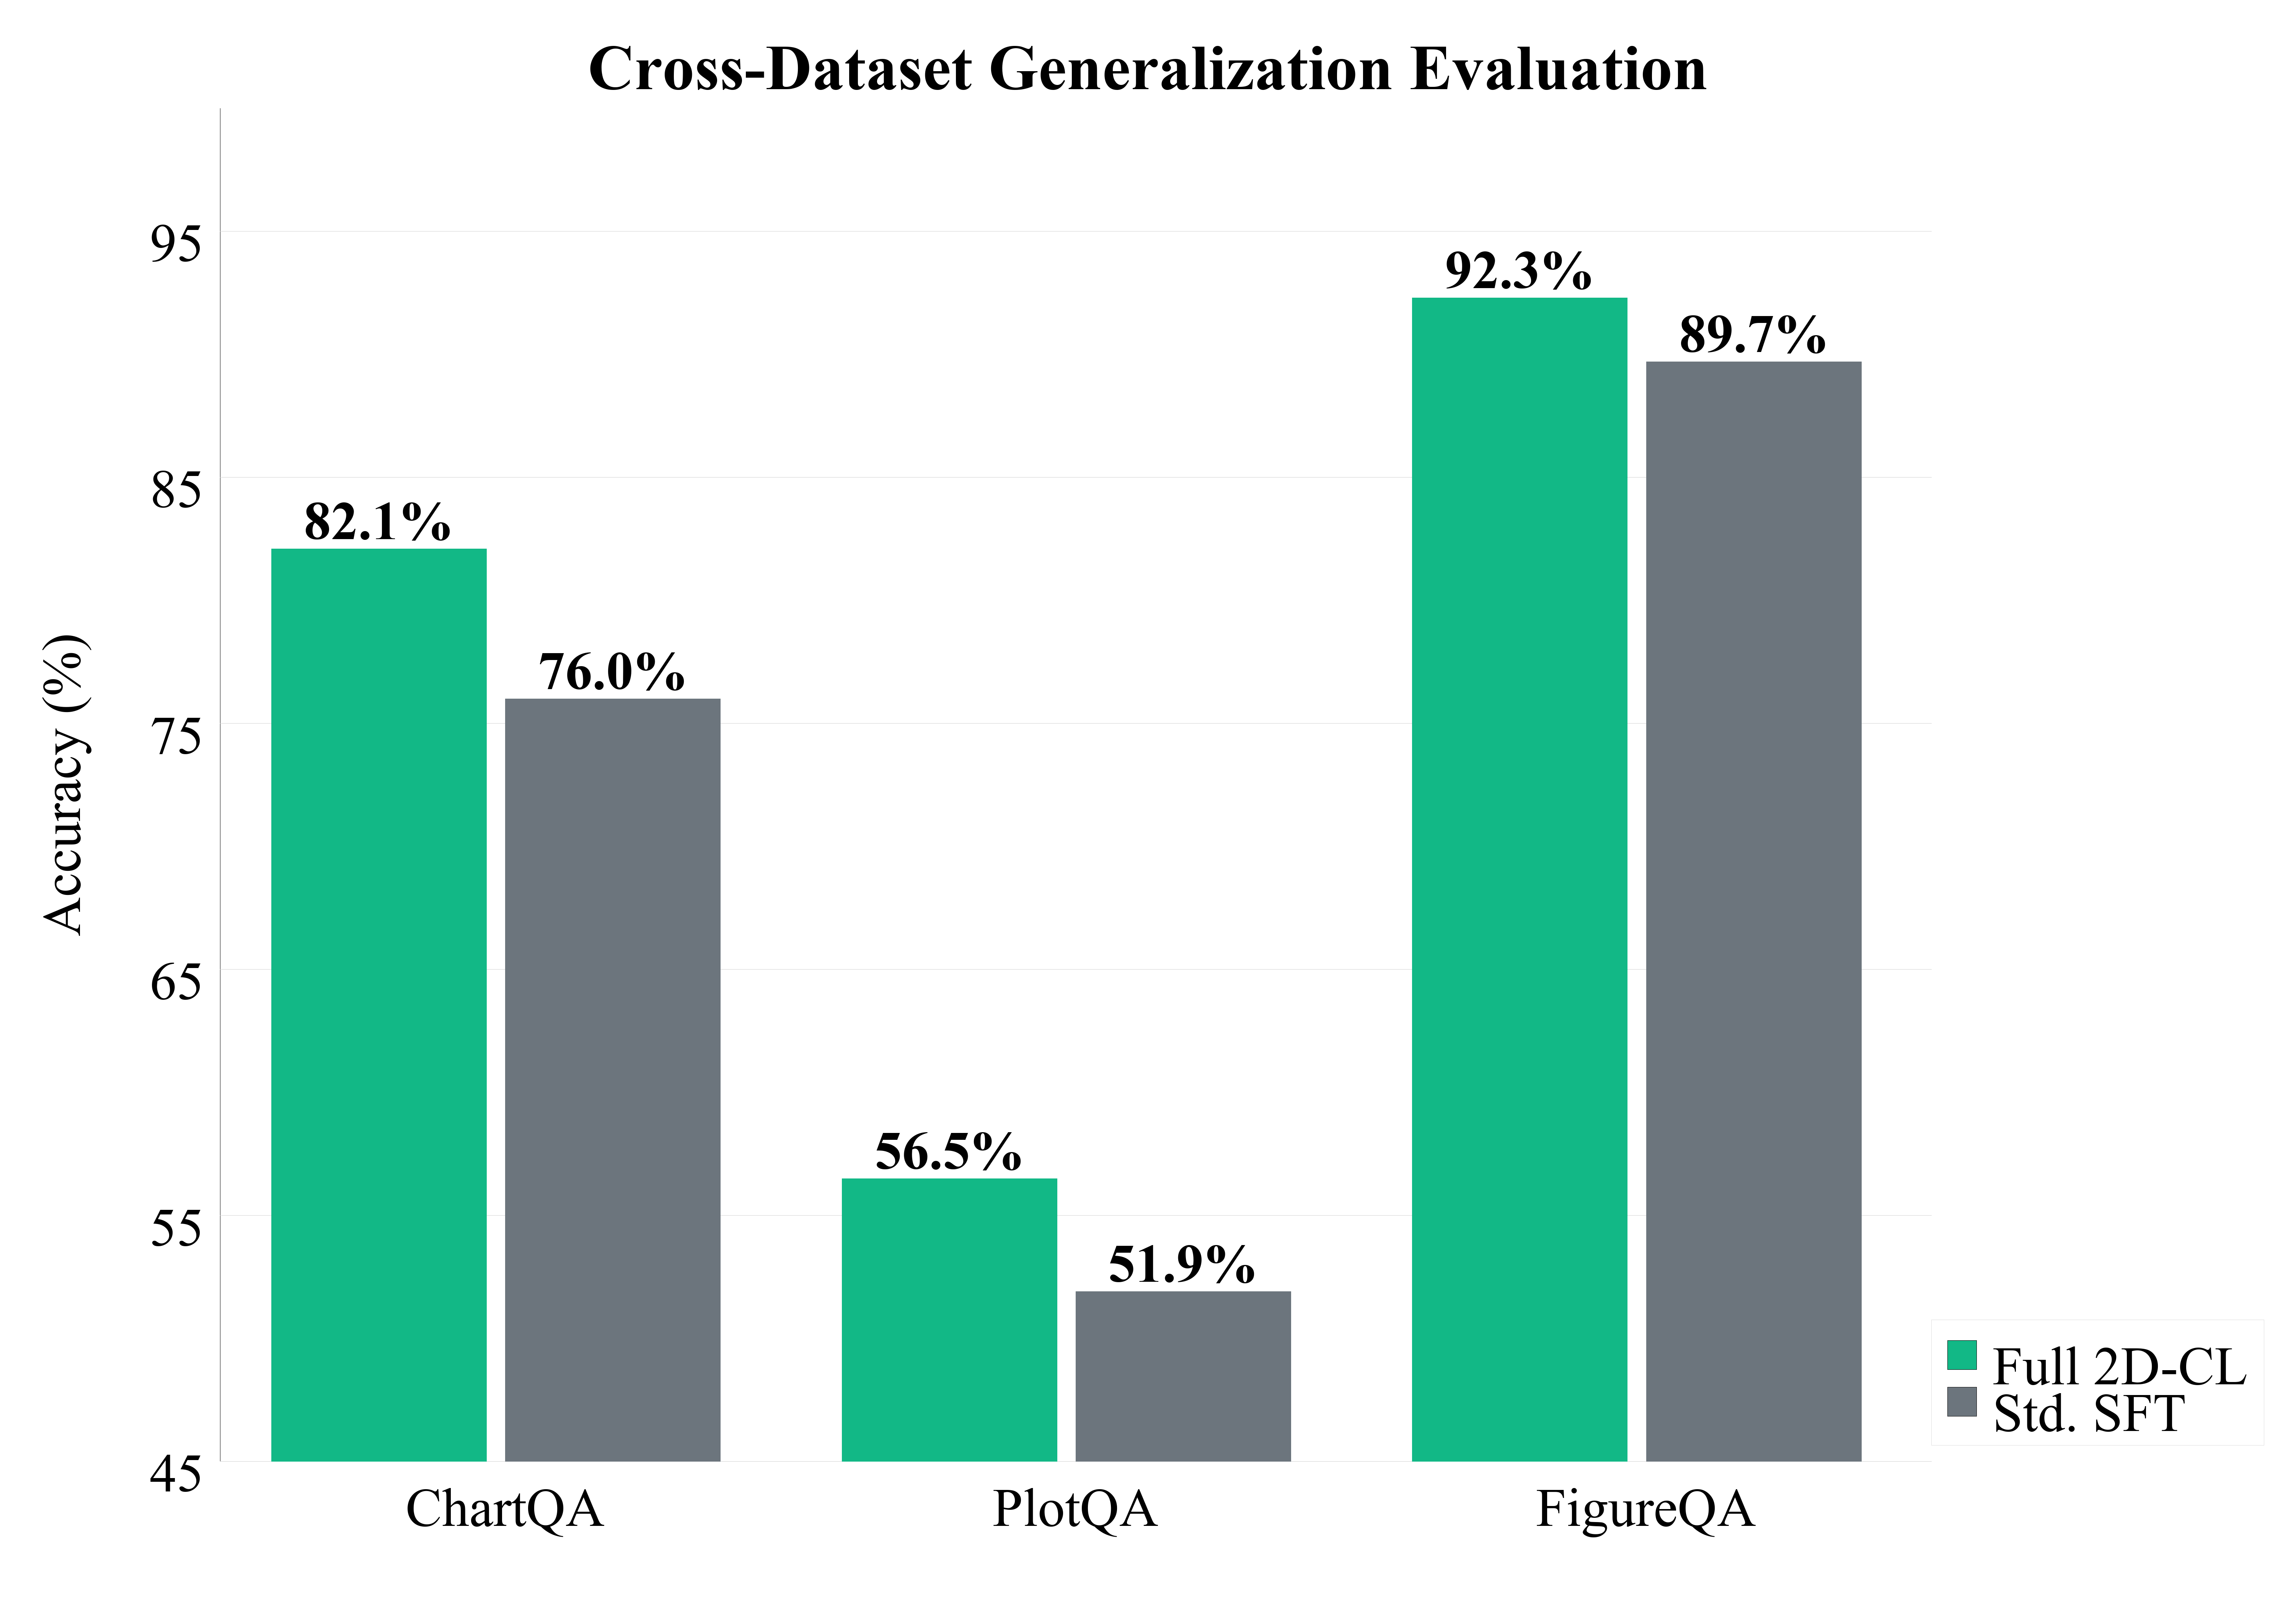
\includegraphics[width=0.32\textwidth]{figs/fig6_cross_dataset_evaluation.png}\label{fig:exp_transfer}}
    \caption{瀹為獙渚濇嵁姒傝銆傚紩鍏?\sar{} 鍚庯紝鐩稿悓瀹氭€ц秼鍔夸粛鐒朵繚鎸侊細姣忎釜璇剧▼缁勪欢閮芥湁浣滅敤锛屽鐩婂彲杩佺Щ鍒颁笉鍚岄骞叉ā鍨嬶紝骞惰兘娉涘寲鍒?ChartQA 涔嬪銆倉
    \label{fig:main_experiments}
\end{figure*}

% TODO-EXP-12: Replace the multi-seed interpretation (mean/std improvements) with real values.
琛▇\ref{tab:seeds} 琛ㄦ槑锛岃繖浜涘鐩婂湪涓嶅悓闅忔満绉嶅瓙涓嬬ǔ瀹氬瓨鍦ㄣ€?
瀹屾暣绯荤粺姣旀爣鍑?SFT 楂?7.40 涓櫨鍒嗙偣锛屾爣鍑嗗樊浠呬负 0.18銆?
鏇村皬鐨勬柟宸鏄庤绋嬬粨鏋勪笉浠呮彁鍗囨渶缁堝噯纭巼锛屼篃鍦ㄤ竴瀹氱▼搴︿笂姝ｅ垯鍖栦簡浼樺寲杩囩▼銆?

% TODO-EXP-13: Replace Table~\ref{tab:models} with real cross-model results.
\begin{table}[!t]
\centering
\small
\begin{tabular}{lccc}
\toprule
\textbf{妯″瀷} & \textbf{Std. SFT} & \textbf{\method{}+\sar{}} & \textbf{$\Delta$} \\
\midrule
Qwen2.5-VL-7B & 76.01 & 83.41 & +7.40 \\
Qwen2.5-VL-3B & 72.41 & 77.58 & +5.17 \\
InternVL2-8B & 77.36 & 81.94 & +4.58 \\
\bottomrule
\end{tabular}
\caption{ChartQA 涓婄殑璺ㄦā鍨嬭瘎娴嬨€傛墍鎻愬嚭妗嗘灦鍚屾椂鎻愬崌浜嗘洿灏忔ā鍨嬪拰鏋舵瀯涓嶅悓鐨勯骞叉ā鍨嬨€倉
\label{tab:models}
\end{table}

% TODO-EXP-14: Replace the cross-model narrative after real model-transfer experiments are done.
琛▇\ref{tab:models} 璇存槑 \method{}+\sar{} 鐨勬敹鐩婂苟涓嶄緷璧栧崟涓€妯″瀷瀹舵棌銆?
涓変釜楠ㄥ共妯″瀷鍧囨湁鎻愬崌锛屽叾涓?Qwen2.5-VL-7B 鐨勭粷瀵规彁鍗囨渶澶э紝鑰岃緝灏忕殑 Qwen2.5-VL-3B 鍜屾灦鏋勪笉鍚岀殑 InternVL2-8B 涔熶繚鐣欎簡鏈夋剰涔夌殑澧炵泭銆?

\subsection{璺敱鍒嗘瀽}
% TODO-EXP-15: Replace Table~\ref{tab:routing} with real routing results.
\begin{table}[!t]
\centering
\small
\begin{tabular}{lcccc}
\toprule
\textbf{鎺ㄧ悊绛栫暐} & \textbf{ChartQA} & \textbf{ChartBench} & \textbf{OpenCQA} & \textbf{骞冲潎} \\
\midrule
Stage 2 only & 81.74 & 70.31 & 64.90 & 72.32 \\
Stage 3 only & 80.68 & 71.24 & 66.11 & 72.68 \\
Stage 4 only & 82.12 & 72.82 & 67.38 & 74.11 \\
Stage 5 only & 78.44 & 69.73 & 65.92 & 71.36 \\
Oracle routing & 84.06 & 75.51 & 70.82 & 76.80 \\
\textbf{Predicted routing (\sar{})} & \textbf{83.41} & \textbf{74.60} & \textbf{69.30} & \textbf{75.77} \\
\bottomrule
\end{tabular}
\caption{璺敱鍒嗘瀽銆俓sar{} 鎭㈠浜嗗ぇ閮ㄥ垎 oracle 璺敱鏀剁泭锛屽苟鍦ㄦ墍鏈夋暟鎹泦涓婄ǔ瀹氫紭浜庝换浣曞浐瀹氬崟闃舵閫傞厤鍣ㄣ€倉
\label{tab:routing}
\end{table}

% TODO-EXP-16: Replace routing-gap, oracle-gap-closing, and routing-distribution claims with real values.
琛▇\ref{tab:routing} 璇存槑浜嗚矾鐢辩殑浠峰€笺€?
娌℃湁鍗曚釜闃舵鑳藉湪鎵€鏈夋暟鎹泦涓婂崰浼橈細闃舵 4 鏄€讳綋鏈€寮哄浐瀹氶€夋嫨锛屼絾骞冲潎浠嶈惤鍚?oracle 璺敱 2.69 涓櫨鍒嗙偣銆?
棰勬祴璺敱鍣ㄦ仮澶嶄簡鍏朵腑 1.66 涓櫨鍒嗙偣锛屽讥鍚堜簡 61.7\% 鐨?oracle 宸窛锛屽悓鏃跺彧浣跨敤杞婚噺鍒嗙被鍣ㄣ€?
鍦?ChartQA 涓婏紝璺敱鍣ㄥ垎鍒负 29\%銆?5\%銆?8\% 鍜?8\% 鐨勬牱鏈€夋嫨闃舵 2銆?銆? 鍜?5锛岃繖涓庣湡瀹炲熀鍑嗛棶棰樿鐩栧绉嶈兘鍔涚被鍨嬬殑鐩磋涓€鑷淬€?

\subsection{鏁版嵁鏁堢巼}
% TODO-EXP-17: Replace Table~\ref{tab:scaling} with real data-scaling results.
\begin{table}[!t]
\centering
\small
\begin{tabular}{lccc}
\toprule
\textbf{璁粌鏁版嵁} & \textbf{Std. SFT} & \textbf{1D-Task} & \textbf{\method{}+\sar{}} \\
\midrule
10\% & 61.80 & 66.42 & 69.73 \\
25\% & 68.91 & 73.46 & 76.84 \\
50\% & 72.73 & 78.38 & 81.02 \\
100\% & 76.01 & 81.27 & 83.41 \\
150\% & 77.18 & 81.96 & 84.03 \\
\bottomrule
\end{tabular}
\caption{ChartQA 涓婄殑鏁版嵁瑙勬ā瀹為獙銆傝绋嬪湪浣庤祫婧愯缃笅灏ゅ叾鏈変紭鍔匡紝涓旈殢鐫€鏁版嵁瑙勬ā澧炲ぇ锛岀浉瀵规帓搴忎繚鎸佷笉鍙樸€倉
\label{tab:scaling}
\end{table}

% TODO-EXP-18: Replace data-efficiency claims and low-resource gain numbers with real values.
琛▇\ref{tab:scaling} 涓殑鏁版嵁瑙勬ā缁撴灉琛ㄦ槑锛屾暟鎹█缂烘椂璇剧▼灏ゅ叾鏈変环鍊笺€?
浠呬娇鐢?10\% 璁粌鏁版嵁鏃讹紝\method{}+\sar{} 宸茬粡姣旀爣鍑?SFT 楂?7.93 涓櫨鍒嗙偣銆?
铏界劧鎵€鏈夋柟娉曢兘浼氶殢鐫€鏁版嵁澧炲鑰屾彁鍗囷紝浣嗘墍鎻愬嚭妗嗘灦鍦ㄦ瘡涓妯′笅閮戒繚鎸佹渶浣筹紝璇存槑鏀剁泭涓嶆槸鏌愪釜鐗瑰畾鏁版嵁閲忎笅鐨勫伓鐒剁幇璞°€?

\subsection{椴佹鎬т笌閿欒鍒嗘瀽}
% TODO-EXP-19: Replace Table~\ref{tab:robustness} with real robustness results.
\begin{table}[!t]
\centering
\small
\begin{tabular}{lccc}
\toprule
\textbf{鎵板姩} & \textbf{Std. SFT 涓嬮檷} & \textbf{\method{} 涓嬮檷} & \textbf{\method{}+\sar{} 涓嬮檷} \\
\midrule
JPEG compression & 6.8 & 4.9 & 4.3 \\
Gaussian blur & 8.1 & 5.6 & 4.8 \\
Low resolution & 7.4 & 5.2 & 4.5 \\
Color jitter & 4.7 & 3.1 & 2.7 \\
Partial occlusion & 9.0 & 6.4 & 5.8 \\
\midrule
Average & 7.2 & 5.0 & 4.4 \\
\bottomrule
\end{tabular}
\caption{ChartQA-C 鍥惧儚鎵板姩涓嬬殑骞冲潎鍑嗙‘鐜囦笅闄嶃€傝绋嬭缁冨拰璺敱閮芥彁鍗囬瞾妫掓€э紝瀹屾暣绯荤粺鐩告瘮鏍囧噯 SFT 灏嗗钩鍧囬€€鍖栧噺灏?2.8 涓櫨鍒嗙偣銆倉
\label{tab:robustness}
\end{table}

% TODO-EXP-20: Replace Table~\ref{tab:error} with real manually labeled error-taxonomy results.
\begin{table}[!t]
\centering
\small
\begin{tabular}{lcc}
\toprule
\textbf{閿欒绫诲瀷} & \textbf{Std. SFT} & \textbf{\method{}+\sar{}} \\
\midrule
Value extraction & 28.4 & 22.9 \\
Arithmetic & 18.7 & 11.6 \\
Multi-step reasoning & 24.9 & 14.8 \\
Answer format & 12.6 & 4.3 \\
Legend/axis mapping & 7.1 & 5.8 \\
Counting/dense perception & 8.3 & 8.0 \\
\bottomrule
\end{tabular}
\caption{瀵?300 涓?ChartQA 澶辫触妗堜緥浜哄伐妫€鏌ュ緱鍒扮殑閿欒鍒嗗竷锛圽%锛夈€傛渶澶ч檷骞呭嚭鐜板湪鎺ㄧ悊鍜屾牸寮忕浉鍏抽敊璇笂锛岃€屽瘑闆嗚鏁颁粛鐒跺叿鏈夋寫鎴樻€с€倉
\label{tab:error}
\end{table}

% TODO-EXP-21: Replace robustness/error-analysis narrative with real drops and observed trends.
琛▇\ref{tab:robustness} 涓殑鎵板姩缁撴灉琛ㄦ槑锛岃绋嬪涔犱笉浠呮彁鍗囧共鍑€鏁版嵁涓婄殑鍑嗙‘鐜囷紝涔熼檷浣庝簡瑙嗚鎵板姩涓嬬殑鎬ц兘閫€鍖栥€?
琛▇\ref{tab:error} 涓殑閿欒鍒嗙被瑙ｉ噴浜嗗師鍥犮€?
鐩告瘮鏍囧噯 SFT锛屾墍鎻愬嚭绯荤粺鏄捐憲鍑忓皯浜嗙畻鏈€佸姝ユ帹鐞嗗拰绛旀鏍煎紡閿欒锛岃繖浜涙鏄?\crs{}銆侀樁娈靛寲鍜岃矾鐢辨墍閽堝鐨勮涓恒€?
鐩稿弽锛屽瘑闆嗚鏁伴敊璇粛鐒跺洶闅撅紝璇存槑鍐荤粨瑙嗚缂栫爜鍣ㄥ湪楂樺害鎷ユ尋鍥捐〃涓婁粛鐒堕檺鍒舵€ц兘銆?

\section{鍒嗘瀽}
\subsection{闃舵涓撻暱}
\sar{} 鑳屽悗鐨勪竴涓牳蹇冪粡楠岃瀵熸槸锛屼笉鍚岃绋嬮樁娈典細鎴愪负涓嶅悓瀛愭妧鑳界殑涓撳銆?
琛▇\ref{tab:stage_performance} 鎶ュ憡浜嗕簲绫诲唴閮ㄤ换鍔′笂鐨勮瘎娴嬬粨鏋溿€?

% TODO-EXP-22: Replace Table~\ref{tab:stage_performance} with real internal stage-specific evaluation results.
\begin{table}[!t]
\centering
\small
\begin{tabular}{lccccc}
\toprule
& \textbf{T1} & \textbf{T2} & \textbf{T3} & \textbf{T4} & \textbf{T5} \\
& Desc. & VQA & Reas. & Vis. & Code \\
\midrule
Baseline & 4.8 & 19.2 & 84.3 & 36.9 & 14.1 \\
Stage 1 & \textbf{25.0} & 11.6 & 72.7 & 43.2 & 11.6 \\
Stage 2 & 5.4 & \textbf{25.1} & 28.7 & 47.4 & 49.2 \\
Stage 3 & 7.1 & 27.2 & \textbf{98.6} & 51.3 & 95.4 \\
Stage 4 & 8.3 & 25.6 & 83.4 & \textbf{82.1} & 50.7 \\
Stage 5 & 4.2 & 23.8 & 63.5 & 75.2 & \textbf{99.2} \\
\bottomrule
\end{tabular}
\caption{闃舵涓撳鍦ㄥ唴閮ㄤ换鍔′笂鐨勮〃鐜般€俆1 涓?BLEU锛孴2--T5 涓哄噯纭巼锛圽%锛夈€傛瘡涓樁娈甸兘鍦ㄥ叾璁捐寮鸿皟鐨勪换鍔℃棌涓婅揪鍒板嘲鍊笺€倉
\label{tab:stage_performance}
\end{table}

% TODO-EXP-23: Replace the stage-specialization interpretation after real internal evaluation is finalized.
琛▇\ref{tab:stage_performance} 涓殑瀵硅浼樺娍寰堟槑鏄俱€?
闃舵 2 鏈€閫傚悎绠€娲佷簨瀹為棶绛旓紝闃舵 3 鏈€閫傚悎鎺ㄧ悊锛岄樁娈?4 鏈€閫傚悎瑙嗚鍒嗘瀽锛岄樁娈?5 鏈€閫傚悎浠ｇ爜閲嶅缓銆?
杩欐鏄?\sar{} 鍦ㄦ帹鐞嗘椂鍒╃敤鐨勭粨鏋勩€?
娌℃湁璺敱鏃讹紝杩欎簺涓撳鍙槸鏈夌敤浣嗕笉渚夸娇鐢ㄧ殑鍓骇鐗╋紱鏈変簡璺敱锛屽畠浠垚涓烘洿濂界郴缁熺殑鍩虹銆?

\subsection{浠ｇ爜鍗虫帹鐞嗙洃鐫ｇ殑浣滅敤}
\begin{figure}[!t]
    \centering
    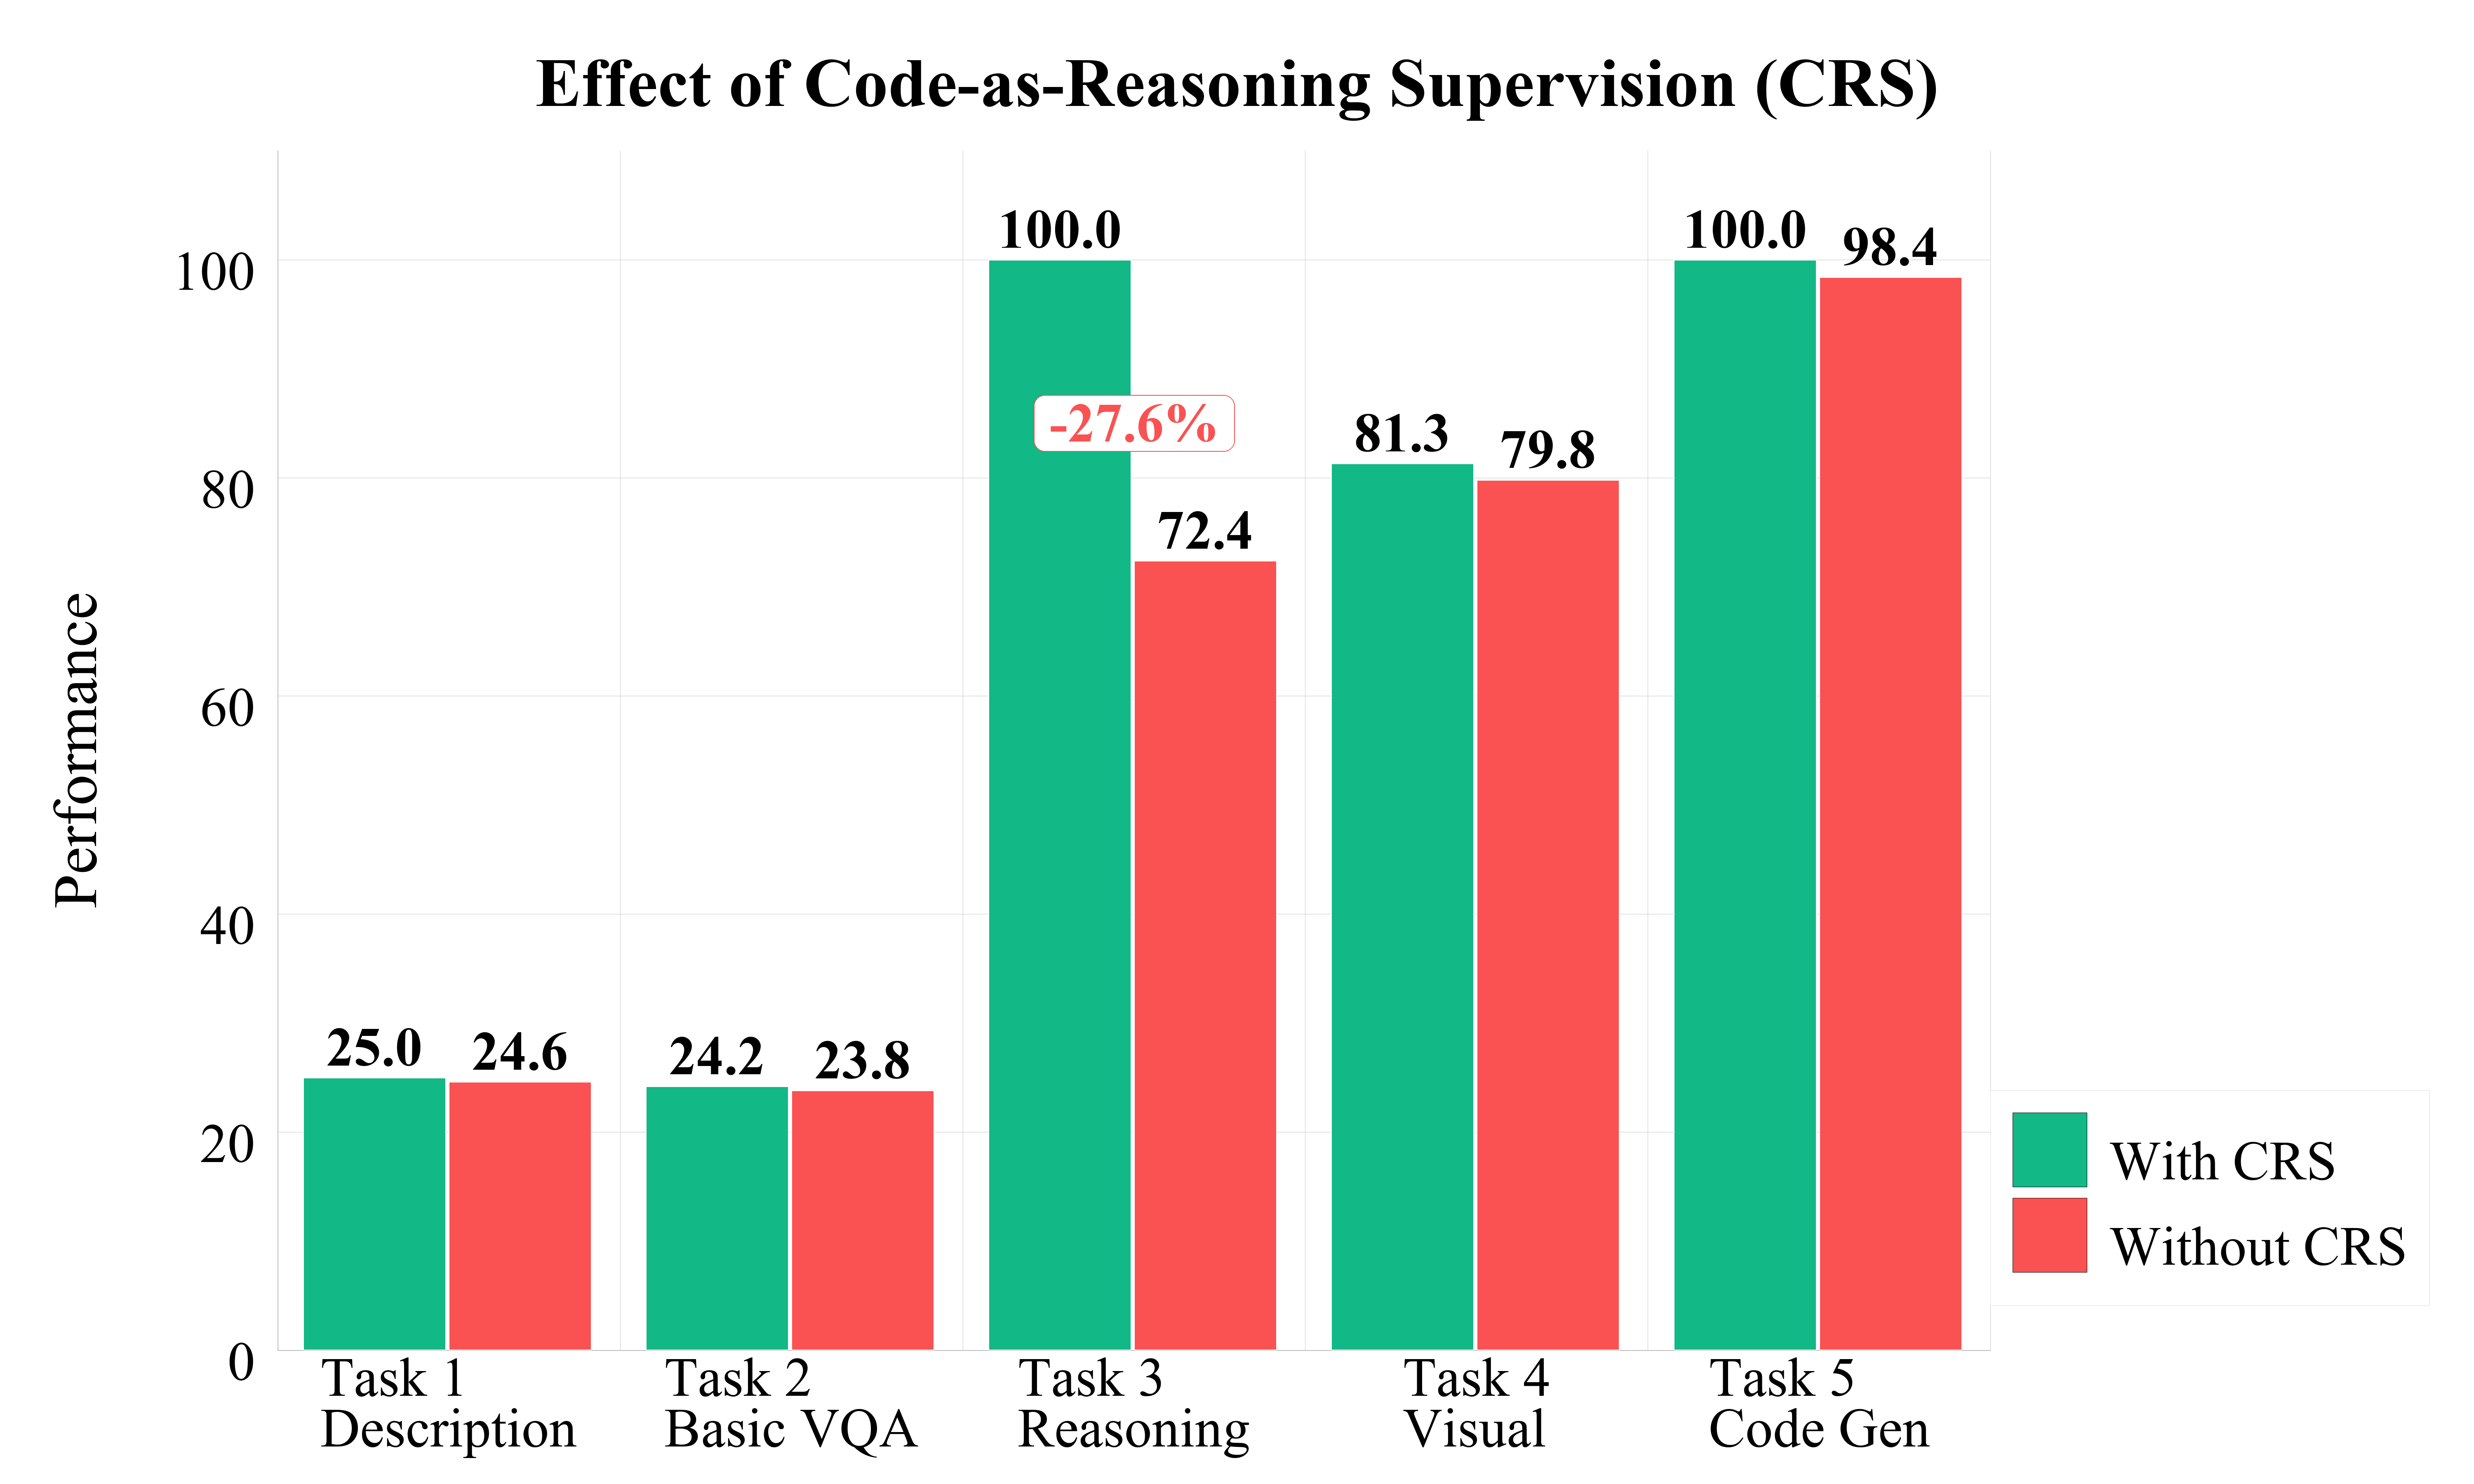
\includegraphics[width=\columnwidth]{figs/fig10_crs_effect.png}
    \caption{\crs{} 瀵规帹鐞嗗瘑闆嗕换鍔＄殑褰卞搷銆傜Щ闄や唬鐮佺洃鐫ｄ富瑕佹崯瀹虫帹鐞嗛樁娈碉紝璇存槑 \crs{} 閽堝鐨勬槸鐗瑰畾鑳藉姏缂哄彛锛岃€屼笉鏄竴鑸€х殑璁粌澧炵泭銆倉
    \label{fig:crs_effect}
\end{figure}

% TODO-EXP-24: Replace CRS-specific drop numbers and reasoning-benchmark claims with real values.
鍥緙\ref{fig:crs_effect} 闅旂浜?\crs{} 鐨勪綔鐢ㄣ€?
鏈€澶т笅闄嶅嚭鐜板湪鎺ㄧ悊瀵嗛泦闂涓婏細绉婚櫎 \crs{} 鍚庯紝鍐呴儴鎺ㄧ悊鍩哄噯鎬ц兘浠?98.6\% 闄嶈嚦 74.3\%銆?
杩欑涓嶅绉板緢閲嶈锛歕crs{} 涓嶅彧鏄鍔犺緭鍑洪暱搴︽垨鍐椾綑鎬э紝鑰屾槸鍦ㄦ暀鎺堜竴绉嶇嫭鐗圭殑璁＄畻琛屼负锛屽苟灏嗗叾杞Щ鍒拌矾鐢卞紡 QA 绯荤粺涓€?

\subsection{涓轰粈涔堥€傞厤鍣ㄧ户鎵块噸瑕亇
% TODO-EXP-25: Recheck this subsection against the final ablation values after experiments finish.
鍦ㄦ垜浠殑娑堣瀺瀹為獙涓紝閫傞厤鍣ㄧ户鎵胯础鐚簡鏈€澶у鐩娿€?
娌℃湁缁ф壙鏃讹紝姣忎釜闃舵瀹炶川涓婇兘鏄竴娆″绔嬬殑寰皟銆?
杩欏闃舵 3 灏ゅ叾鏈夊锛屽洜涓哄畠蹇呴』浠呭嚟 1,775 涓帹鐞嗘牱鏈悓鏃跺涔犺瑙夊畾浣嶅拰澶氭鎺ㄧ悊銆?
鏈変簡缁ф壙锛岄樁娈?3 鍙互鍋囪浣庡眰鍥捐〃瀹氫綅宸茬粡寤虹珛锛屼粠鑰屾妸瀹归噺鐢ㄤ簬璁＄畻锛岃€屼笉鏄噸鏂板涔犳劅鐭ャ€?

\subsection{闅惧害鍙潬鎬
% TODO-EXP-26: Replace difficulty-reliability statistics (agreement, deviation, ordering comparison) with real values.
涓洪獙璇?\dacds{}锛屾垜浠汉宸ユ爣娉?300 涓牱鏈殑浜旂骇闅惧害鏍囩锛屽苟涓庡熀浜?LLM 鐨勫垎鏁版瘮杈冦€?
涓€鑷寸巼涓?82.7\%锛屽钩鍧囩粷瀵瑰亸宸负 0.41 涓瓑绾с€?
鏇撮噸瑕佺殑鏄紝鎺掑簭鏈韩纭疄鏈変綔鐢細鍦ㄧ浉鍚岄樁娈电粨鏋勪笅锛岀敱鏄撳埌闅炬帓搴忕ǔ瀹氫紭浜庣敱闅惧埌鏄擄紙80.34\%锛夊拰闅忔満鎺掑簭锛?1.27\%锛夈€?
杩欑‘璁や簡 \dacds{} 鐨勬敹鐩婃潵鑷湁鎰忎箟鐨勬牱鏈帓搴忥紝鑰屼笉鏄瘎鍒嗚繃绋嬩腑鐨勫櫔澹般€?

\subsection{瀹氭€ф渚媫
% TODO-EXP-27: Replace this qualitative summary with real selected cases after manual case curation.
瀹氭€ф鏌ヤ腑鍙嶅鍑虹幇涓ょ妯″紡銆?
绗竴锛岃矾鐢辩郴缁熺粡甯镐慨澶嶆爣鍑?SFT 鐨勭瓟妗堟牸寮忛敊璇細杩囧幓浼氳Е鍙戝啑闀胯В閲婄殑闂琚噸瀹氬悜鍒伴樁娈?2锛屽苟浠ュ熀鍑嗘湡鏈涚殑绠€娲佺簿纭尮閰嶆牸寮忓洖绛斻€?
绗簩锛岀畻鏈瘑闆嗛棶棰樼粡甯歌璺敱鍒伴樁娈?3锛屾ā鍨嬬粰鍑虹畝鐭絾璁＄畻涓€鑷寸殑绛旀锛屽弽鏄犱簡閫氳繃 \crs{} 瀛﹀埌鐨勬帹鐞嗕範鎯€?
涓庢鍚屾椂锛屾寔缁瓨鍦ㄧ殑閿欒闆嗕腑鍦ㄥ瘑闆嗚鏁版垨寰堝皬鐨勮瑙夋爣璁颁笂锛岀獊鏄句簡鍐荤粨瑙嗚缂栫爜鍣ㄧ殑灞€闄愩€?

\section{璁ㄨ}
% TODO-EXP-28: Recalibrate the discussion after all experimental evidence is finalized.
瀹屾暣缁撴灉鏀寔鐨勭粨璁哄苟涓嶅彧鏄熀鍑嗗垎鏁版彁鍗囥€?
瀵逛簬鍥捐〃鐞嗚В鑰岃█锛孿emph{璁粌缁撴瀯} 鏈韩灏辨槸閲嶈璁捐鍙橀噺銆?
鎵€鎻愬嚭璇剧▼鎻愬崌浜嗕紭鍖栫ǔ瀹氭€с€佹暟鎹晥鐜囧拰杩佺Щ鑳藉姏锛岃€岃矾鐢辫〃鏄庡闃舵涓撻暱鍙互鎴愪负浼樺娍锛岃€屼笉鏄儴缃茶礋鎷呫€?

杩欎簺澧炵泭涔熸彮绀轰簡缁勪欢涔嬮棿鐨勫垎宸ャ€?
闃舵鍖栦笌缁ф壙閫愭鏋勫缓鑳藉姏锛沑crs{} 寮哄寲鏄惧紡璁＄畻锛沑dacds{} 骞虫粦闃舵鍐呬紭鍖栵紱\sar{} 鍒欏皢涓撻暱杞寲涓哄疄闄呮帹鐞嗐€?
杩欑鍒嗚В鏈夊姪浜庤В閲婁负浠€涔堝畬鏁存鏋跺悓鏃朵紭浜庢爣鍑?SFT 鍜屼竴缁磋绋嬨€?

涓庢鍚屾椂锛屽墿浣欓敊璇垎甯冭〃鏄庯紝骞堕潪鎵€鏈夌摱棰堥兘鑳戒粎闈犺缁冪粍缁囪В鍐炽€?
鍦ㄥ瘑闆嗘垨浣庡垎杈ㄧ巼鍥捐〃涓婄殑鎰熺煡閿欒浠嶇劧瀛樺湪锛岃繖璇存槑鏈潵宸ヤ綔搴斿皢璇剧▼瀛︿範涓庢洿寮虹殑鍥捐〃鎰熺煡瑙嗚缂栫爜鍣ㄦ垨鍖哄煙绾х洃鐫ｇ粨鍚堣捣鏉ャ€?

\section{缁撹}
鎴戜滑鎻愬嚭浜嗛潰鍚戝浘琛ㄧ悊瑙ｇ殑 \fullmethod{}锛岃妗嗘灦娌夸换鍔″鏉傚害鍜屾牱鏈毦搴︾粍缁囧涔犮€?
璇ユ柟娉曠敱 \crs{} 鎻愪緵鏄惧紡鍙墽琛屾帹鐞嗙洃鐫ｏ紝骞剁敱 \dacds{} 鎻愪緵闅惧害鎰熺煡鏍锋湰鎺掑簭銆?
涓轰簡璁╂墍寰楅樁娈典笓瀹跺湪閮ㄧ讲鏃跺彲鐢紝鎴戜滑杩涗竴姝ユ彁鍑?\sar{}锛屼竴绉嶄负姣忎釜鏌ヨ閫夋嫨鏈€鍚堥€備笓瀹剁殑杞婚噺璺敱妯″潡銆?

% TODO-EXP-29: Replace conclusion-level summary results with final real numbers and claims.
鍦?ChartQA銆丳lotQA銆丗igureQA銆丆hartBench 鍜?OpenCQA 涓婏紝鎵€鎻愬嚭绯荤粺绋冲畾浼樹簬鏍囧噯 LoRA 寰皟鍜屽己鍗曢樁娈靛熀绾裤€?
鍦?ChartQA 涓婏紝\method{}+\sar{} 浠呯敤 12K 鍚堟垚鏍锋湰杈惧埌 83.41\%锛屽悓鏃舵彁鍗囦簡椴佹鎬с€佹暟鎹晥鐜囧拰鎺ㄧ悊鍙敤鎬с€?
杩欎簺缁撴灉琛ㄦ槑锛屽浜庡浘琛ㄧ悊瑙ｈ繖绫诲妯℃€佹帹鐞嗕换鍔★紝缁勭粐妯″瀷 \emph{濡備綍} 瀛︿範锛屽彲鑳戒笌鎵╁睍妯″瀷 \emph{浠庝粈涔坿 鏁版嵁涓涔犲悓鏍烽噸瑕併€?

\section*{灞€闄愭€
鏈爺绌朵粛鏈夎嫢骞插眬闄愩€?

\paragraph{鍚堟垚璁粌鍒嗗竷銆倉
灏界杩佺Щ缁撴灉浠や汉榧撹垶锛岃绋嬩富瑕佸湪鍚堟垚鍥捐〃涓婅缁冦€?
鍏锋湁寮傚父甯冨眬銆佸祵濂楁爣娉ㄦ垨棰嗗煙鐗瑰畾绾﹀畾鐨勭湡瀹炲浘琛ㄤ粛鍙兘閫犳垚鍒嗗竷鍋忕Щ銆?

\paragraph{璺敱鐩戠潱銆倉
\sar{} 渚濊禆鐢变繚鐣欐暟鎹瀯閫犵殑 oracle 璺敱鏍囩銆?
灏界璺敱鍣ㄨ交閲忎笖鏈夋晥锛屾洿鍘熷垯鍖栫殑绔埌绔仈鍚堝涔犱笓瀹跺拰璺敱鐨勫舰寮忓彲鑳借繘涓€姝ユ彁鍗囨€ц兘銆?

\paragraph{鍥捐〃绫诲瀷瑕嗙洊銆倉
鎴戜滑鍏虫敞浜旂甯歌鍥捐〃绫诲瀷銆?
鐑浘銆佹鍩哄浘銆佸湴鍥惧拰 3D 鍥剧瓑鏇村箍娉涚殑鍙鍖栧舰寮忎粛涓嶅湪鏈枃鑼冨洿鍐呫€?

\paragraph{璇█鑼冨洿銆倉
鎵€鏈夊疄楠屽潎涓鸿嫳鏂囥€?
澶氳瑷€鍥捐〃鐞嗚В浠嶆槸寮€鏀鹃棶棰樸€?

\appendices
\section{璁粌缁嗚妭}
\paragraph{鏁版嵁闆嗘瀯鎴愩€倉
鍥緙\ref{fig:dataset_dist} 鍙鍖栦簡鍚堟垚璁粌鏁版嵁鐨勬瀯鎴愩€?
鍥捐〃绫诲瀷鍒嗗竷澶ц嚧鍧囪　锛屽叾涓煴鐘跺浘鍜屾姌绾垮浘鐣ュ浜庨潰绉浘銆?
闅惧害绛夌骇鎸夎璁″亸鍚戠畝鍗曟牱鏈紝杩欏弽鏄犱簡璇剧▼瀛︿範鎬濇兂銆?

\begin{figure}[!t]
    \centering
    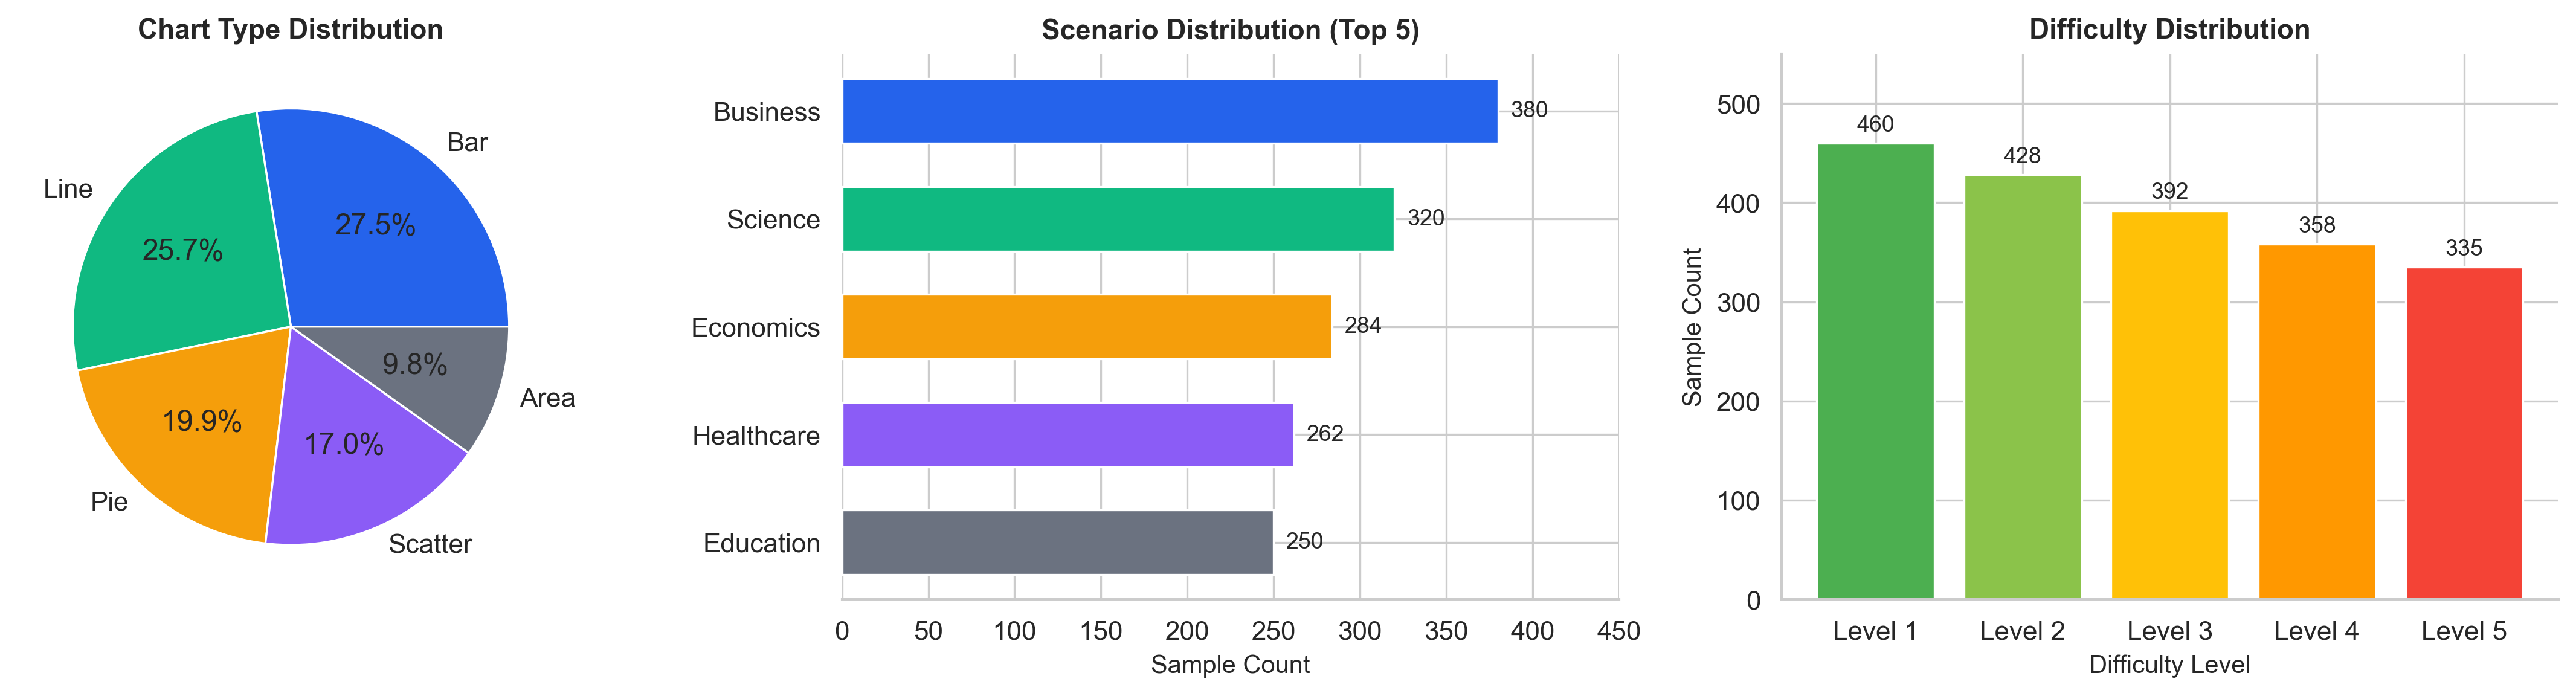
\includegraphics[width=\columnwidth]{figs/fig11_dataset_distribution.png}
    \caption{鍚堟垚璁粌鏁版嵁鍒嗗竷銆傦紙a锛夊浘琛ㄧ被鍨嬨€傦紙b锛夊満鏅被鍒€傦紙c锛夐毦搴︾瓑绾с€倉
    \label{fig:dataset_dist}
\end{figure}

\paragraph{瓒呭弬鏁般€倉
琛▇\ref{tab:hyperparams} 鍒楀嚭浜嗗悇闃舵瓒呭弬鏁般€?
闃舵 5 浣跨敤鏇撮暱鐨勬渶澶у簭鍒楅暱搴︿互瀹圭撼浠ｇ爜杈撳嚭銆?

\begin{table}[!t]
\centering
\small
\begin{tabular}{lccccc}
\toprule
& \textbf{S1} & \textbf{S2} & \textbf{S3} & \textbf{S4} & \textbf{S5} \\
\midrule
Learning Rate & 1e-4 & 5e-5 & 3e-5 & 3e-5 & 2e-5 \\
Epochs & 10 & 10 & 10 & 10 & 10 \\
Batch Size & 16 & 16 & 16 & 16 & 16 \\
Max Length & 2048 & 2048 & 2048 & 2048 & 4096 \\
Warmup Ratio & 0.05 & 0.05 & 0.05 & 0.05 & 0.05 \\
Weight Decay & 0.01 & 0.01 & 0.01 & 0.01 & 0.01 \\
LoRA Rank & 8 & 8 & 8 & 8 & 8 \\
LoRA Alpha & 16 & 16 & 16 & 16 & 16 \\
LoRA Dropout & 0.1 & 0.1 & 0.1 & 0.1 & 0.1 \\
\bottomrule
\end{tabular}
\caption{璇剧▼璁粌鐨勮秴鍙傛暟銆倉
\label{tab:hyperparams}
\end{table}

\paragraph{璁粌鍔ㄦ€併€倉
琛▇\ref{tab:training_dynamics} 鎬荤粨浜嗗悇闃舵浼樺寲杩囩▼銆?
澶у鏁伴樁娈靛湪鍓嶄袱鍒颁笁涓?epoch 鍐呰揪鍒版渶缁堟€ц兘鐨?90\%锛岃鏄庣户鎵挎彁渚涗簡鑹ソ鐨勫垵濮嬪寲銆?

\begin{table}[!t]
\centering
\small
\begin{tabular}{lccccc}
\toprule
& \textbf{S1} & \textbf{S2} & \textbf{S3} & \textbf{S4} & \textbf{S5} \\
\midrule
\# Samples & 1,775 & 1,775 & 1,775 & 5,327 & 1,775 \\
Initial Loss & 2.34 & 1.18 & 0.86 & 0.58 & 0.42 \\
Final Loss & 0.667 & 0.381 & 0.268 & 0.173 & 0.109 \\
Reduction (\%) & 71.5 & 67.7 & 68.8 & 70.2 & 74.0 \\
Epochs to 90\% & 3 & 2 & 2 & 4 & 2 \\
Wall-clock (h) & 3.6 & 2.7 & 2.5 & 9.6 & 2.5 \\
\bottomrule
\end{tabular}
\caption{鍚勯樁娈佃缁冨姩鎬併€傞樁娈?4 鏈€鑰楁椂锛屽洜涓哄叾鏍锋湰鏁扮害涓哄叾浠栭樁娈电殑涓夊€嶃€倉
\label{tab:training_dynamics}
\end{table}

\section{闄勫姞缁撴灉}
\paragraph{璺敱鏁堢巼銆倉
% TODO-EXP-30: Replace routing-efficiency numbers and latency claims with real deployment measurements.
琛▇\ref{tab:efficiency} 鎶ュ憡浜嗛樁娈佃矾鐢辩殑閮ㄧ讲鎴愭湰銆?
璺敱鍣ㄦ瘡涓牱鏈粎澧炲姞 5.7 ms 寤惰繜锛屽苟涓旈伩鍏嶅姞杞藉涓ぇ鍨嬪畬鏁存ā鍨嬶紝鍥犱负鎵€鏈変笓瀹跺叡浜悓涓€涓喕缁撻骞诧紝浠呭湪杞婚噺 LoRA 鍙傛暟涓婁笉鍚屻€?

\begin{table}[!t]
\centering
\small
\begin{tabular}{lcc}
\toprule
\textbf{鎸囨爣} & \textbf{鏈€浣抽樁娈祡 & \textbf{\method{}+\sar{}} \\
\midrule
Latency / sample (ms) & 184.2 & 189.9 \\
Extra routing cost (ms) & --- & 5.7 \\
Adapter storage (MB) & 77 & 308 \\
Backbone copies & 1 & 1 \\
\bottomrule
\end{tabular}
\caption{閮ㄧ讲鏁堢巼銆傝矾鐢卞櫒澧炲姞鐨勫欢杩熷緢灏忥紝涓旂敱浜庢帹鐞嗘椂鍙垏鎹㈣交閲?LoRA 閫傞厤鍣紝绯荤粺浠嶇劧瀹炵敤銆倉
\label{tab:efficiency}
\end{table}

\paragraph{缁勪欢璐＄尞銆倉
% TODO-EXP-31: Replace Table~\ref{tab:component_detail} with real component-drop values.
琛▇\ref{tab:component_detail} 鎶ュ憡浜嗕粠瀹屾暣绯荤粺涓Щ闄ゅ悇缁勪欢鏃?ChartQA 鍑嗙‘鐜囩殑涓嬮檷銆?

\begin{table}[!t]
\centering
\small
\begin{tabular}{lcc}
\toprule
\textbf{绉婚櫎缁勪欢} & \textbf{Acc. (\%)} & \textbf{鐩稿瀹屾暣绯荤粺鐨?$\Delta$} \\
\midrule
\textit{Full \method{}+\sar{}} & \textit{83.41} & --- \\
\midrule
w/o Adapter Inheritance & 77.86 & $-5.55$ \\
w/o Task Staging & 79.18 & $-4.23$ \\
w/o CRS & 80.11 & $-3.30$ \\
w/o Difficulty Ordering & 81.27 & $-2.14$ \\
w/o Router & 82.12 & $-1.29$ \\
\midrule
Standard LoRA SFT & 76.01 & $-7.40$ \\
\bottomrule
\end{tabular}
\caption{鍦?ChartQA 涓婏紝浠ヤ粠瀹屾暣绯荤粺绉婚櫎鍚勭粍浠跺悗鐨勬€ц兘涓嬮檷琛￠噺缁勪欢璐＄尞銆倉
\label{tab:component_detail}
\end{table}

\paragraph{澶氫换鍔＄敾鍍忋€倉
% TODO-EXP-32: Replace Table~\ref{tab:task_profile} with real internal multi-task comparison results.
琛▇\ref{tab:task_profile} 姣旇緝浜嗚绋嬭缁冧笌鏍囧噯 SFT 鍦ㄤ簲绫诲唴閮ㄤ换鍔′笂鐨勮〃鐜般€?
鏈€澶у鐩婂嚭鐜板湪鎺ㄧ悊鍜屼唬鐮佺浉鍏充换鍔′笂锛岃繖涓?\crs{} 鍜岄樁娈靛寲鑳藉姏鏋勫缓鐨勮璁″姩鏈轰竴鑷淬€?

\begin{table}[!t]
\centering
\small
\begin{tabular}{lcc}
\toprule
\textbf{浠诲姟绫诲瀷} & \textbf{\method{}} & \textbf{Standard SFT} \\
\midrule
T1: Description (BLEU) & 25.0 & 12.8 \\
T2: Basic VQA (Acc.) & 25.1 & 18.4 \\
T3: Reasoning (Acc.) & 98.6 & 60.2 \\
T4: Visual Analysis (Acc.) & 82.1 & 55.4 \\
T5: Code Generation (Acc.) & 99.2 & 63.1 \\
\bottomrule
\end{tabular}
\caption{鍐呴儴浠诲姟鏃忎笂鐨勬€ц兘銆傝绋嬪涔犲鎺ㄧ悊瀵嗛泦鑳藉姏鐨勬彁鍗囨渶鏄庢樉銆倉
\label{tab:task_profile}
\end{table}

\bibliographystyle{IEEEtran}
\bibliography{references}

\end{CJK*}
\end{document}

